\section{Introduction}
\label{representation_analysis_introduction}
In this chapter we will proceed at analyzing the representations inferred by the architectures developed in chapter \ref{chapter_implementation_testing}. Our aim will be to probe and inspect them in the attempt to evaluate if they possess some of the functional characteristics proper of attributed incentive salience. Indeed, despite the predictive properties assessed in chapter \ref{chapter_implementation_testing} are a necessary condition for a good approximation of the motivational state of an individual (see section \ref{comp_framework}, they are surely not sufficient. 

Differently from what has been done in chapter \ref{chapter_implementation_testing}, we will conduct our investigation using  a combination of dimensionality reduction, unsupervised learning and visual analyses. We will focus on evaluating differences and similarities between the representations derived from the RNN architecture and its improved version (i.e., RNN with environmental and game events covariates) as they represent the final versions of our methodology that more c. 

We will first briefly introduce the idea that ANNs are able to learn a manifold structure of the data (which reflects the objective function that they are trying to optimize) by embedding it in a high dimensional latent representation. We will also clarify the procedure we followed for extracting these representations using our ANN architectures. Subsequently we will illustrate how it is possible to visualize their manifold structures by means of appropriate dimensionality reduction technique.  After that we will define which type of functional characteristics we expect these structures to show  and which differences we expect to see between the two architectures. Finally by means of unsupervised learning we will conduct a series of exploratory partition analysis on the representations generated by the ANN. This will be done in the attempt to individuate profiles able to map what inferred by the models back to the observable behavioural space. The steps of the analysis pipeline used in this chapter are illustrated in Figure \ref{fig: pipeline_inspect}.
\begin{figure}[!htb]
  \centering
  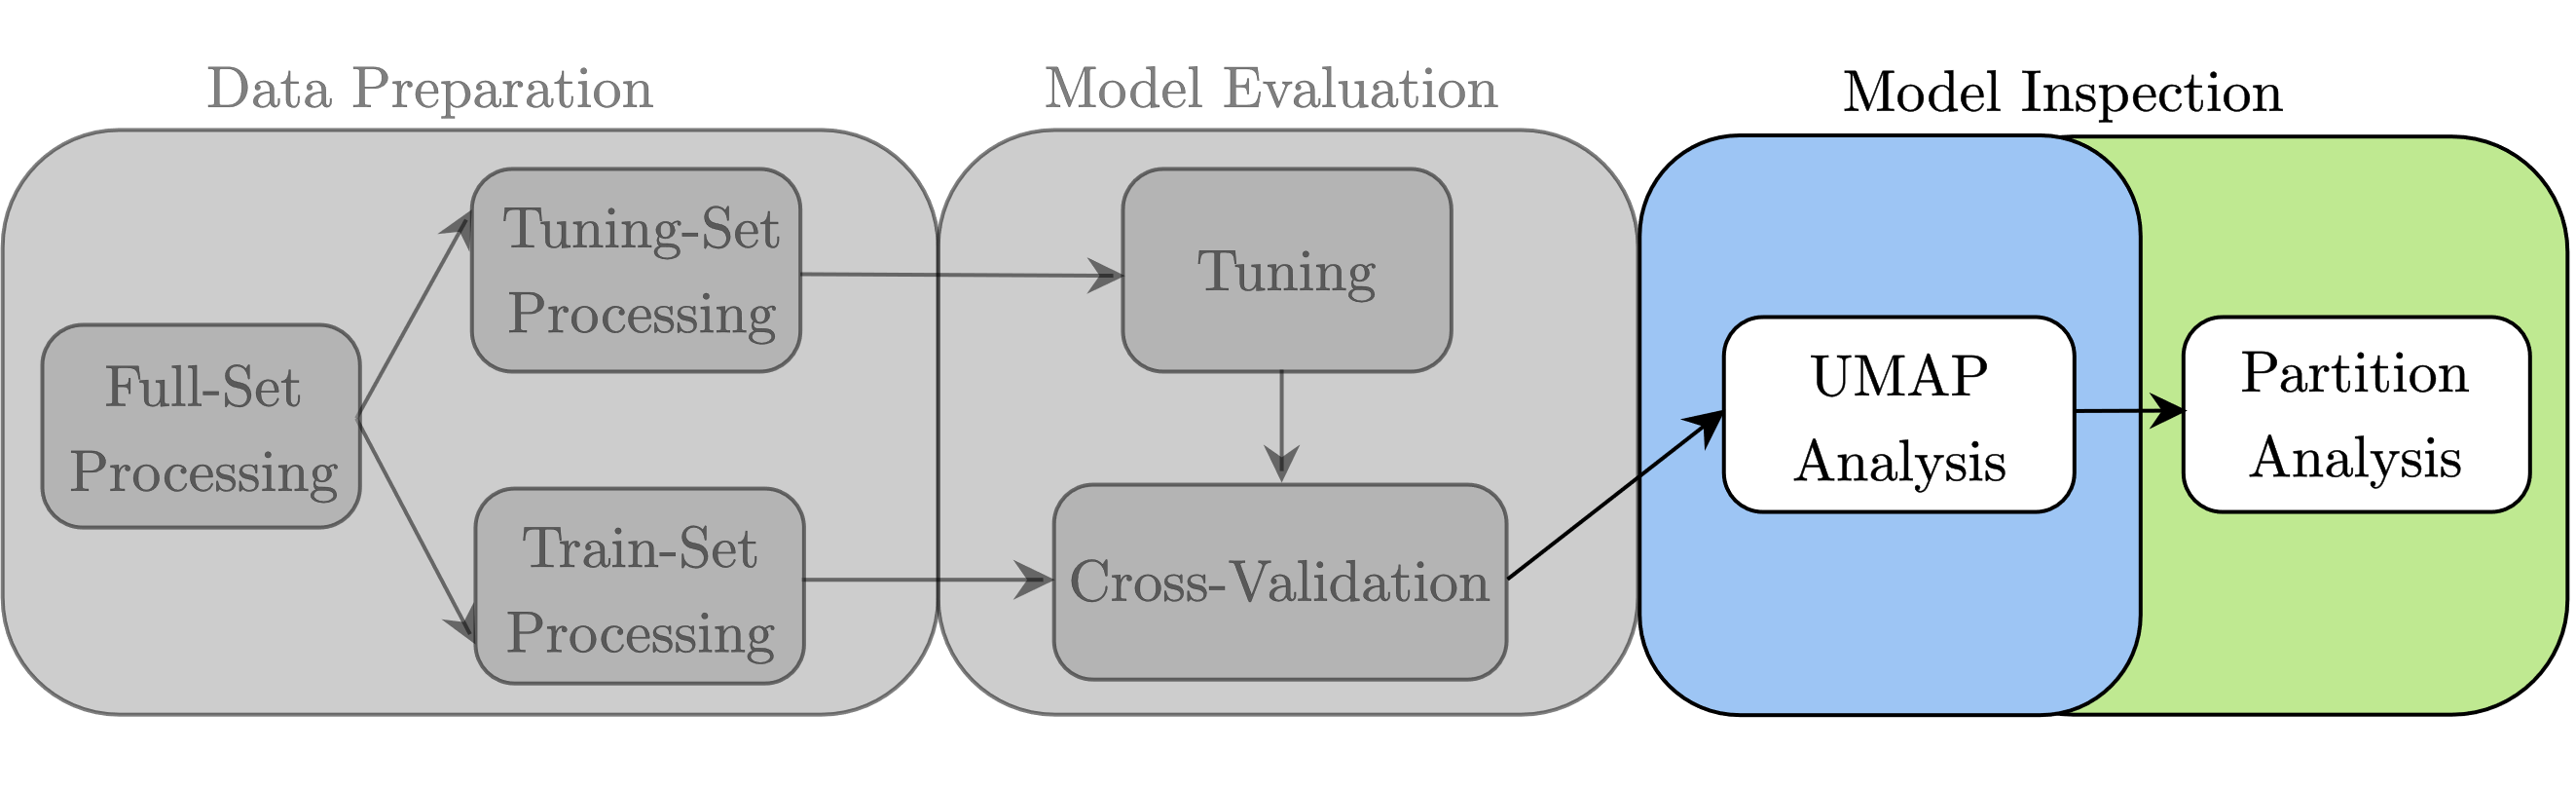
\includegraphics[width=\textwidth]{images/chapter_4/pipeline_inspect.png}
    \caption[\textbf{Representation analysis experimental pipeline}]{Arrows indicate the flow of the pipeline. Big coloured blocks are major pipeline steps, white rectangles indicate sub-tasks within each step. This experimental pipeline stems directly from the "Model Evaluation" stage outline in figure \ref{fig: pipeline_eval}.}
    \label{fig: pipeline_inspect}
\end{figure}

\section{Extracting and Visualizing the Latent Representation}
\label{extract_visulize}

\subsection{Neural Networks, manifolds and embeddings}
\label{manifold_learning_embed}
As we mentioned in section \ref{chapter_theory_modelling}, when trying to approximate a certain function, ANNs would do it so by mapping the input they receive to a lower dimensional manifold. By moving along this manifold it is possible to reach inputs with different characteristics and observe how they relate with the output produced by the model.

Despite the manifold structure learned by the model might be intrinsically low dimensional, it is usually stored (or better, it is "embedded"), in a (potentially sparse) high dimensional representation \cite{bengio2017deep}. This representation has usually less degrees of freedom than the original input but it is still challenging to parse from a human perspective. Simplifying, this can be compared to storing the "instructions" on how to extract the low dimensional manifold from the input in a distributed fashion across all the parameters of the ANNs. In our case if we look at Figures \ref{fig: rnn_2} and \ref{fig: rnn_env_even}, the portion of the architecture marked in red should, once fitted to the input data, provide us with the relevant "instructions" on how to obtain an approximation of the manifold structure describing the level of attributed incentive salience (see chapter \ref{chapter_theory_modelling} for the theoretical reasons behind this assertion).

As illustrated in sections \ref{artificial_neural_networks} and \ref{manifold_learning}, since an ANNs can be thought as directed acyclic computational graphs (DAGs), to obtain the representation produced at any point of a specific architecture it is sufficient to pass a given input through all the operations performed before that point. Figure \ref{fig: repr_extr} illustrate the process for the RNN architecture presented in section \ref{model_architecture_2}.

\begin{figure}[!htb]
  \centering
  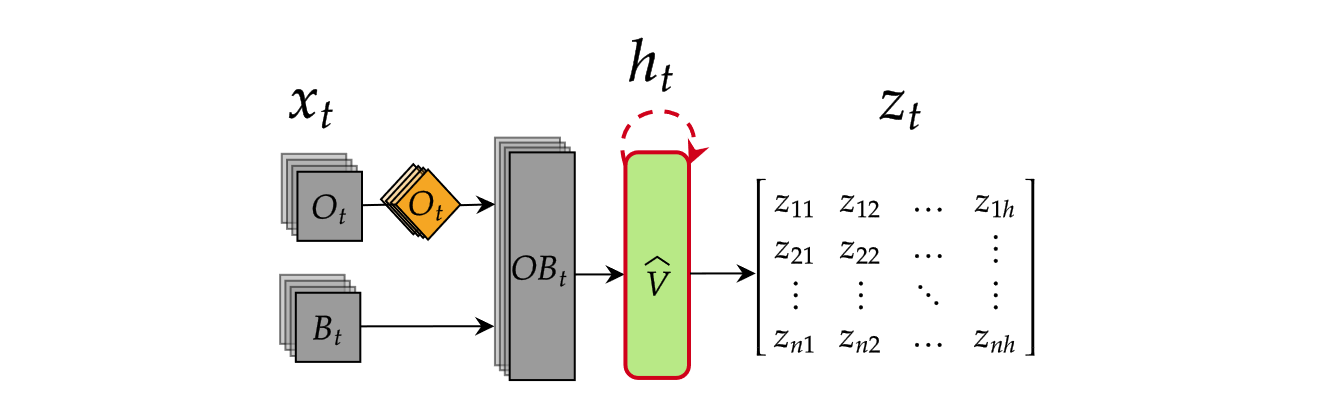
\includegraphics[width=\textwidth]{images/chapter_4/representation_extractor.png}
    \caption[\textbf{The procedure for generating latent representations generated by an ANN}]{Orange and green shapes represent respectively embedding and LSTM layers. Embedding layers are a type of feedforward layers specifically designed for dealing with categorical inputs \cite{chollet2015keras}. Gray shapes indicate operations with no learnable parameters, such as tensor instantiation and concatenation. The orange transparent shape indicate the concatenation of a single embedding with multiple tensors. Stacked, transparent colouring indicates arrays with a sequential structure. Straight and curved arrows refer to the presence of feed-forward or recurrent information flow. The red highlight shows the portion of the model we hypothesize is inferring an approximation of attributed incentive salience. Given inputs $O \in \mathbb{Z}^{N \times t}$ and $B \in \mathbb{R}^{N \times t \time 5}$, the matrix $Z_t \in \mathbb{R}^{N \times h}$ represents the $h$ dimensional (where $h$ is the number of hidden units in the recurrent layer) representation generated by the ANN at time $t$ after all operations in its underlying computational graph have been performed.}
    \label{fig: repr_extr}
\end{figure}

Borrowing the terminology from the self-supervised deep learning literature \cite{bengio2017deep} we call this truncated version of the original architecture encoder. Encoders can be thought as functions (which parameters have been learned during the fitting procedure) mapping input data onto the manifold space learned by the original architecture. From now on, we will use the term encoder for referring to the two considered architectures truncated at the point of the last shared recurrent operation.

\subsection{Dimensionality Reduction and Manifold Approximation}
\label{dim_reduction}
If we look at figure \ref{fig: repr_extr} we can see that with increasing size of $h$ it becomes more and more challenging to inspect the representation generated by the encoder. However If we recall from section \ref{manifold_learning_embed} the intrinsic dimensionality for this representation should be much smaller. In the case of a latent state like attributed incentive salience this could be as small as one dimensional, two if we consider the nature of the rewarding object (see section \ref{motivation_hist} and Figure \ref{fig: vect_mot} in particular). 

In this view a convenient approach for inspecting the shape of the learned manifold would be to perfrom some form of dimensionality, Principal Component Analysis (PCA) \cite{pearson1901liii} would be the most reasonable approach given the straightforward interpretation of the derived components. However the choice of which algorithm to chose is not necessarily that straightforward. 

Looking at figure \ref{fig: swiss_ambient}, we can see the example of a dataset constituted by three separate (the separation aspect is important and will be further in section \ref{functional_properties}) point clouds (denoted by different colours) in a three dimensional ambient space (the space in which a low dimensional manifold might be embedded). Red and green clouds are examples of the synthetic Swiss Roll dataset \cite{scikit-learn}, while the blue cloud is a simple random projection of a square. Both datasets are basically equivalent (i.e. intrinsically two dimensional with the main dimension highlighted by the colour gradient) but differ in their layout in ambient space: the square is linear while the Swiss roll warps in a non linear fashion.

\begin{figure}[!htb]
  \centering
  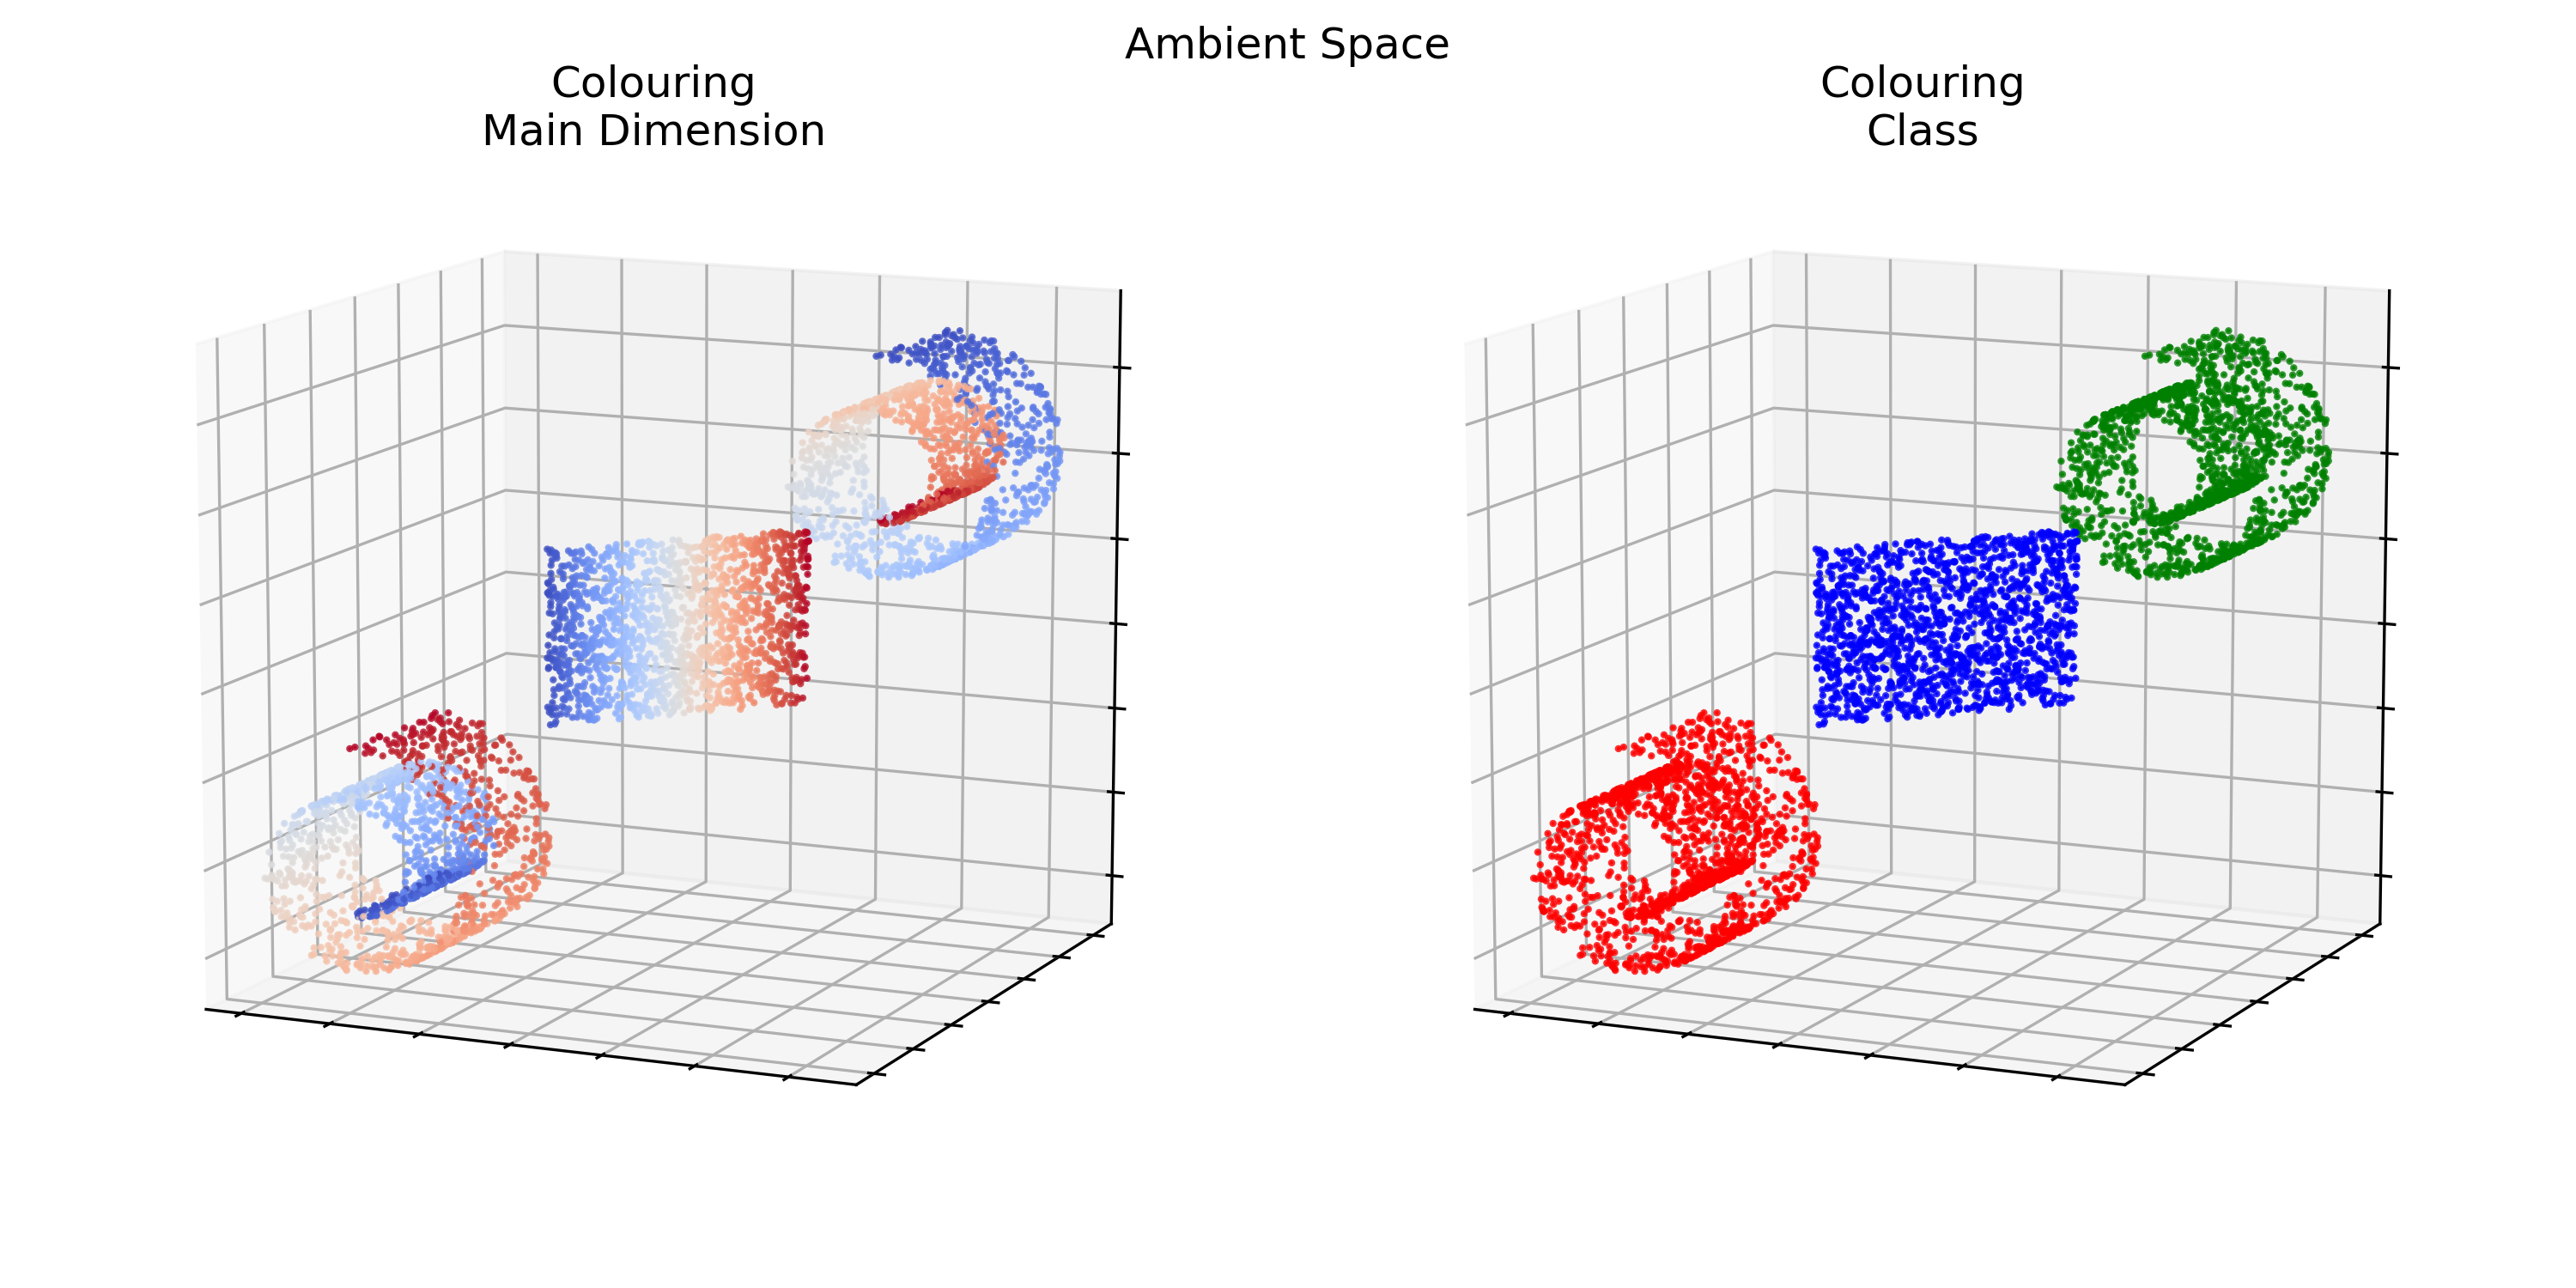
\includegraphics[width=\textwidth]{images/chapter_4/ambient.png}
    \caption[\textbf{Swiss rolls and square in ambient space}]{The figure show three point clouds which are intrinsically 2-dimensional (a Swiss roll and a square) embedded in a 3-dimensional ambient space. In both panels the X, y and z axes represent the coordinate of the ambient space. The colours in the first panel indicates the main dimension of variation while those in the second panel simply identify membership of points to a specific cloud.}
    \label{fig: swiss_ambient}
\end{figure}

Figure \ref{fig: swiss_reduce} show the dimensionality reduction performed by PCA along with an alternative non-linear dimensionality reduction approach: the Uniform Manifold Approximation and Projection (UMAP) \cite{2018arXivUMAP}. 

\label{dim_reduction}
\begin{figure}[!htb]
  \centering
  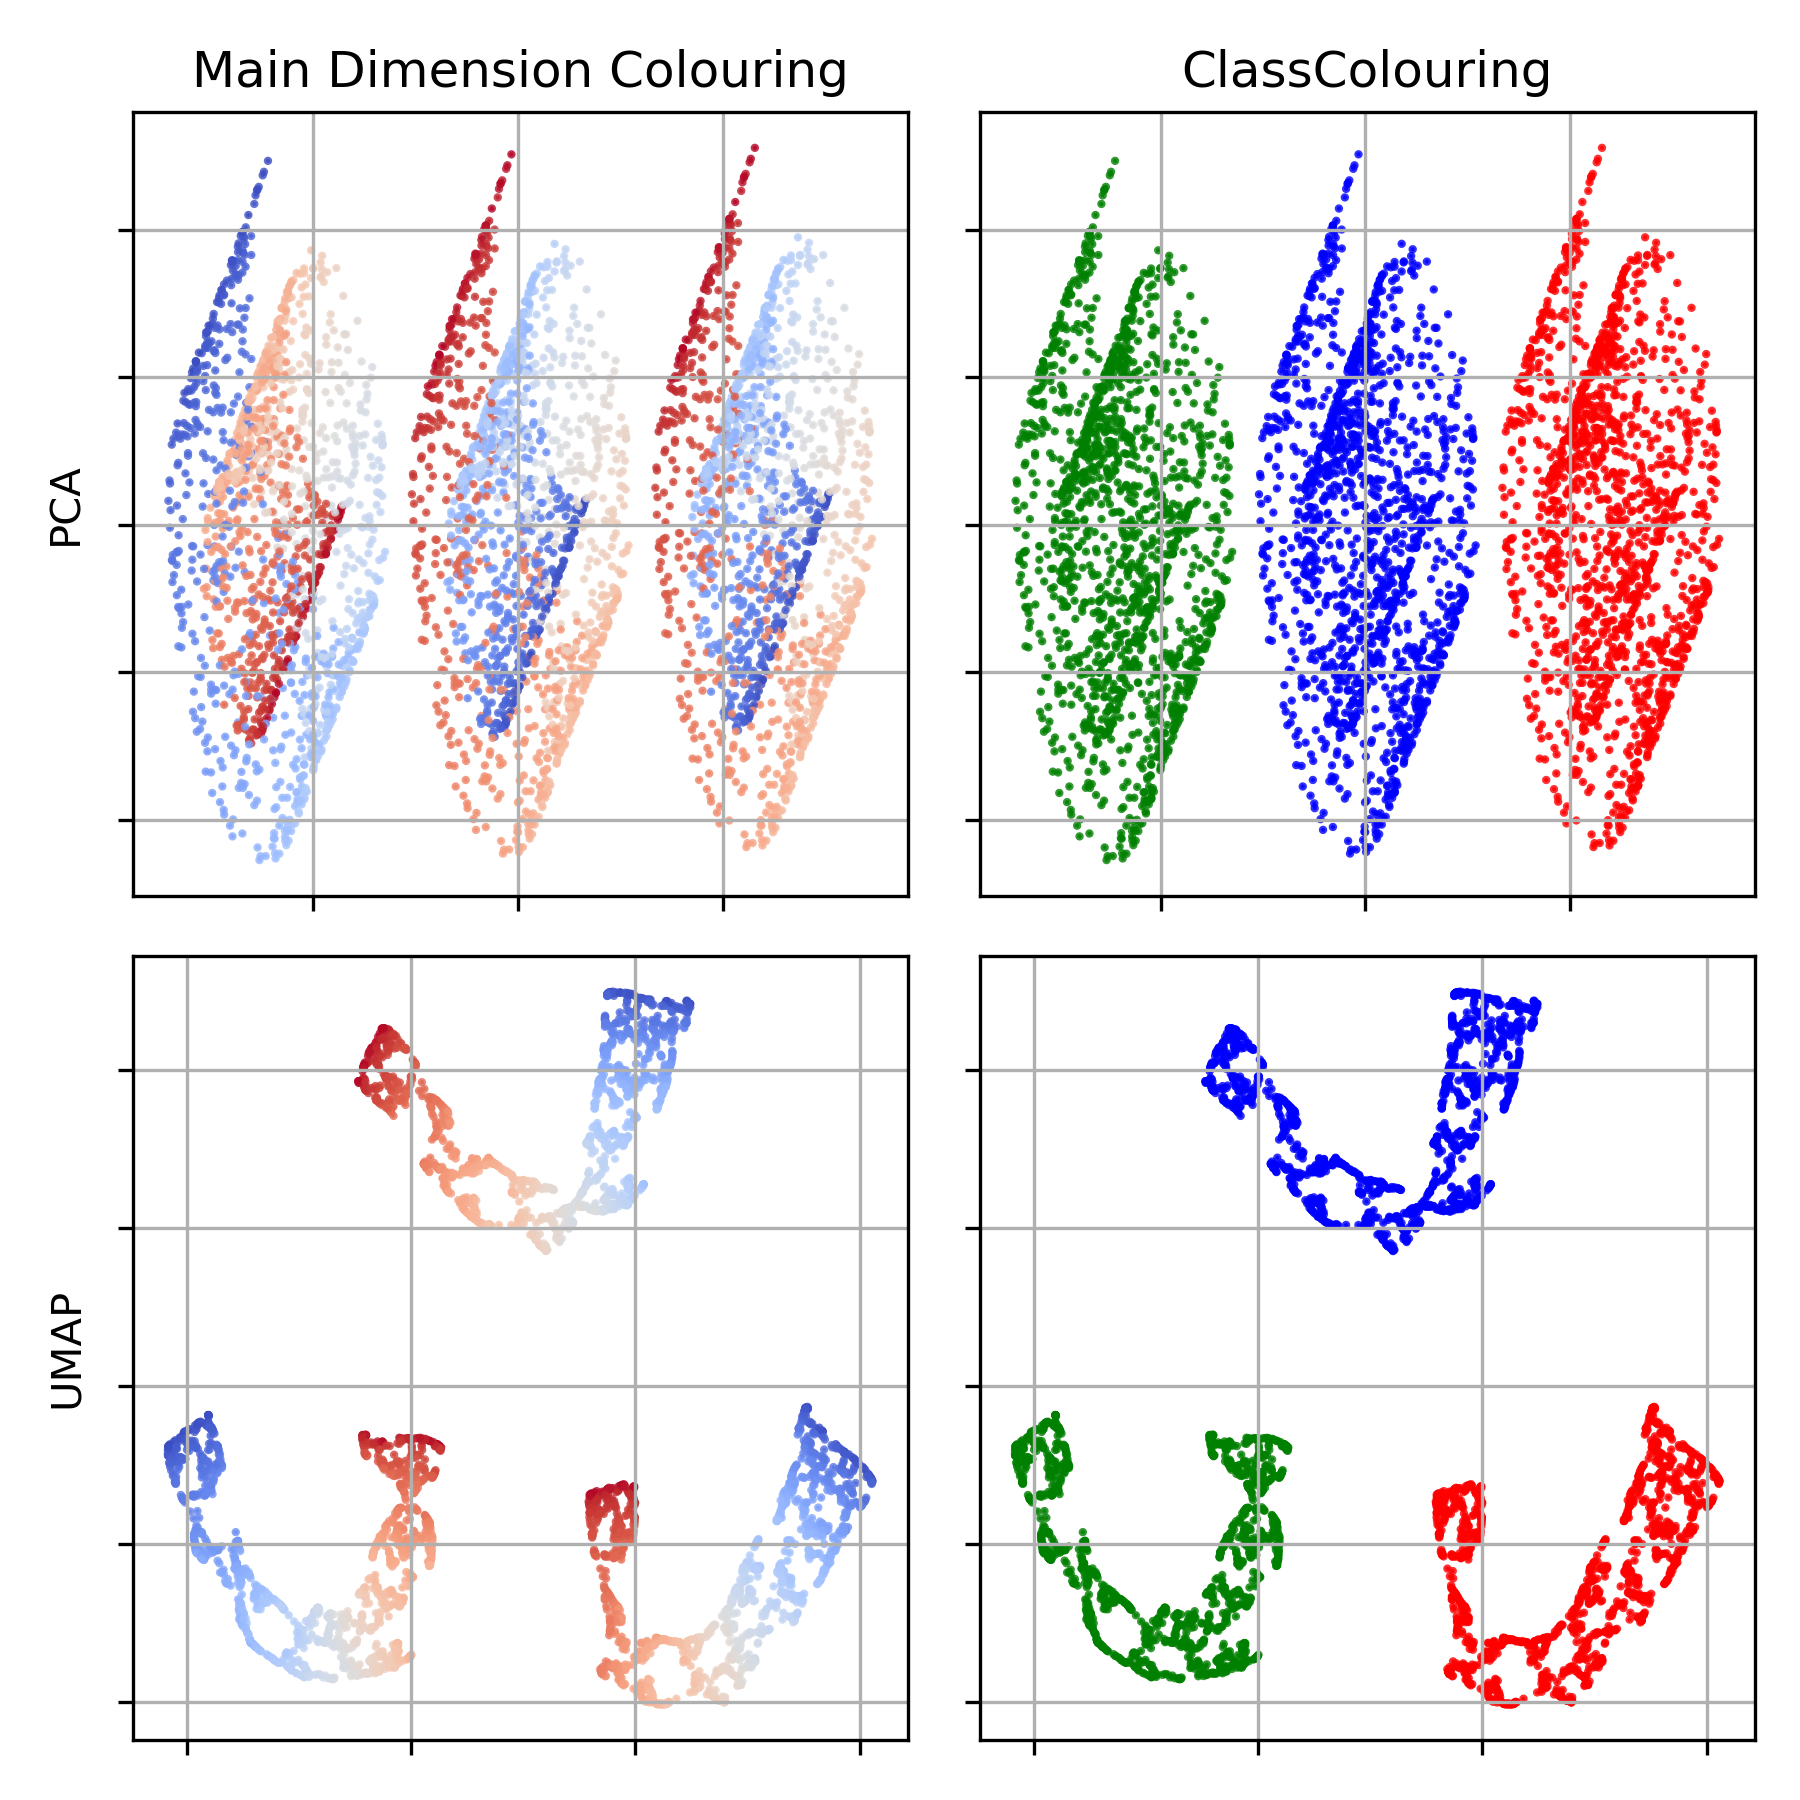
\includegraphics[width=0.7\textwidth]{images/chapter_4/reduced.png}
    \caption[\textbf{PCA and UMAP reduction of Swiss roll and square}]{The figure show the reduction of the 3-dimensional point clouds to a 2-dimensional plane. The panels in the first row show the reduction produced by PCA while those in the second row show the reduction produced by UMAP. In all panels the x, y axes represent the components extracted by PCA and UMAP. The colours in the two columns again indicate the main dimension of variation and the membership of points to a specific cloud.}
    \label{fig: swiss_reduce}
\end{figure}

The UMAP algorithm is a dimensionality reduction technique based on manifold learning. Given a high dimensional dataset, UMAP first infers its topological structure by means of a k-nearest neighbours graph and then, using stochastic gradient descent, attempts to structurally reproduce it in a lower dimensional space (two or three for visualization purposes) \cite{2018arXivUMAP}. Despite being a still local algorithm, compared to other similar approaches (for example, the t-distributed Stochastic Neighbor Embedding \cite{van2008visualizing}),  UMAP has the ability to better preserve the global structure of the original data. Moreover, when given datasets that are sequential in natures (like those produce by the recurrent part of our architecture) UMAP is able to include this characteristics during the optimization process \footnote{See \cite{alignedumap} for implementation details.} generating lower dimensional representations that are aligned over time. 

What we observe in Figure  \ref{fig: swiss_reduce} is that both techniques manage to keep the separation between point clouds, but PCA, differently from UMAP, struggles to faithfully represent the the intrinsic structure of the data. This toy example is particularly relevant in our case as the representation generated by ANNs are by design highly non-linear. This will be made evident in the next section where we will proceed at visualizing the representation learned by our ANNs architecture.

\section{Representation Analysis}
\label{representation_analysis}
In order to support our idea that the representation learned by the different architectures could be interpreted as an approximation of the latent states generated by incentive salience, we carried out a series of qualitative analyses. If our intuitions were in the right right direction we expected the representations inferred by the architectures to exhibit a series of characteristics and functional properties:
\begin{enumerate}
    \item To possess an intrinsic dimensionality that is much smaller than the observed one.
    \item To be able to effectively distinguish between different game objects.
    \item To be able to effectively distinguish between individuals based on the expected intensity of their future interactions with the considered game objects.
    \item To be able to show the two aforementioned characteristics consistently over time.
\end{enumerate}

The characteristics mentioned above are concerned with a general validation of the properties of the latent representation for all the considered architectures, however we also wanted to understand if the included covariates altered and improved the generated representation.  Hence, we preceded at inspecting also the representation extracted by the encoder derived from the improved version of the RNN architecture. 

The procedure followed for extracting the latent representations was the same for all architectures. First, we re-fitted all models on a random sample (i.e. 90\%) of the validation-set following the same procedures specified in chapter \ref{chapter_implementation_testing}. Then, we created 6 encoders using the approach illustrated in paragraph \ref{manifold_learning_embed} and Figure \ref{fig: repr_extr}. Two were used for extracting the representations expected to approximate the level of attributed incentive salience (red highlights in Figures \ref{fig: rnn_2} and \ref{fig: rnn_env_even)}. One for extracting the same type of representation inferred however by the MLP architecture (this was done for comparative purposes). And  three for extracting the intermediate representations generated by the improved version of the RNN architecture (i.e. those relative to the behavioural, environmental and game events input). Subsequently, we passed the remaining portion of the validation-set (i.e. 10\%) as an input to the encoders, producing arrays of shape $(N \times T \times h)$ with $N$ being the number of considered individuals, $h$ the number of hidden units in the last layer of the encoder and $T$ the number of observed interactions for the considered individuals. This means that all representations have been generated with out-of-sample data. In our case, since all architectures were of type sequence-to-sequence we were able to investigate not just the properties of the generated representation at specific point in time, but also the dynamics underlying their evolution. 

To summarize, we can say that each considered encoder was tasked to generate a high dimensional representation where distance could be interpreted as similarity between individuals with respect to the expected intensity of their future interactions with a specific game object (see the manifold hypothesis of attributed incentive salience presented in paragraph \ref{manifold_rep_incentive_salience}). Dimensionality reduction was then used for approximating the intrinsic manifold structure of these representations on a 2 dimensional plane in order to allow for qualitative visual analysis. 

The reduction to a 2D plane was done leveraging the UMAP algorithm. The algorithm first inferred the topological structure of the produced representations by computing the cosine distance in a local neighborhood of 1000 points with a minimum distance of 0.8. The projection on a two dimensional plane was then achieved by running the optimization part of the algorithm for 2000 iterations. The choice of a large neighborhood and minimum distance was made to better capture the global structure of the manifold \footnote{See \cite{umapwebs} for a visualization of the effects of these hyperparameters in UMAP.}. 

In order to gather an understanding on the characteristics of the function used for generating the latent representations, we also conducted a set of purely exploratory investigations of the relationship between hidden units' activation in the recurrent layers and the predictions produced by the model. To quantify the strength of the observed relationship we employed the Maximal Information Coefficient (MIC) \cite{reshef2011detecting}, a measure of mutual information that can quantify both linear and non-linear association between variables. The MIC can assume values between 0 to 1 with 1 corresponding to a perfect association. 

We adopted the implementation of UMAP provided McInnes \textit{et. al.} \cite{mcinnes2018umap-software} while the MIC was computed using the python library minepy \cite{albanese2013minerva}. Visualizations were produced using the python libraries matplotlib \cite{hunter2007matplotlib} and seaborn \cite{waskom2021seaborn}.

\subsection{Validating the Functional Properties of the Inferred Latent Representation}
\label{functional_properties}
As a first thing we proceeded at investigating if the assumption about the intrinsic dimensionality of the latent representation could be considered reasonable. Looking at figure \ref{cross_corr_act}

\begin{figure}[!htb]
\centering
\includegraphics[width=0.5\textwidth]{images/chapter_4/corr_matrices.png}
\caption[\textbf{Cross-correlation analysis of the hidden units activation of the RNN architecture}]{Each panel shows the cross correlation between the activity of the RNN's artificial neurons in all the game objects going from $t1$ to $t4$. The y and x axes are symmetrical and identifies the RNN artificial neurons while the coloured cells report the Spearman's Rho correlation coefficient for the activation of each pair of neurons. White cells represent combinations for which the correlation coefficient resulted lower than 0.05.}
\label{cross_corr_act} 
\end{figure}

we can observe consistent patterns of cross-correlation for the activity of the hidden units constituting the latent representation, suggesting the presence of redundancy. In order to support this finding and for gathering a general sense of the intrinsic dimensionality of the embedded manifold, we  conducted a Principal Component Analysis (PCA). Despite PCA and UMAP working under radically different assumptions and mechanisms, we thought this could provides us with a general idea of how much variance we would be able to capture by reducing the representation to a lower dimensional space. 

\begin{figure}[!htb]
\centering
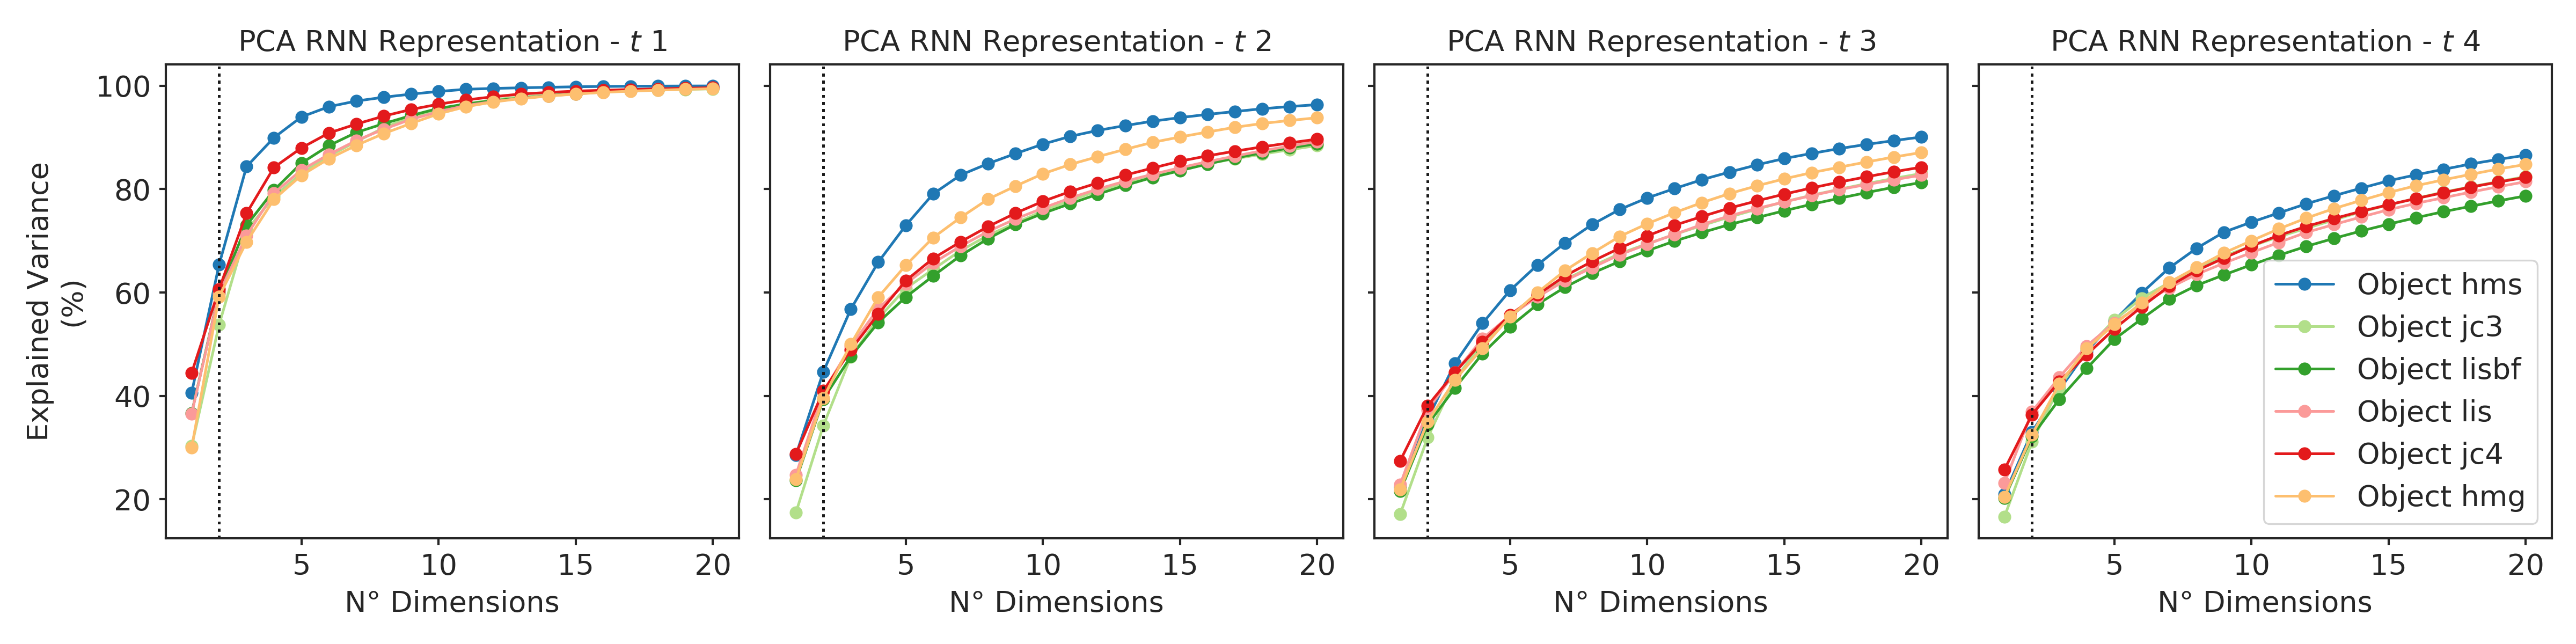
\includegraphics[width=\textwidth]{images/chapter_4/pca_embedding.png}
\caption[\textbf{Principal component analysis of the hidden units activation of the RNN architecture }]{The panel shows the percentage of explained variance by considering 2 to 20 principal components for each game object going from $t1$ to $t4$. The y axis indicates the percentage of explained variance while the x axis the number of principal components considered.}
\label{pca_emb} 
\end{figure}

Looking at figure \ref{pca_emb} we can see that two principal components can explain a large portion of variance in the representation generated by the RNN. Precisely, across game contexts the first two principal components were able to explain from 30 to 60\% of the variance, with maximum explanatory power around 6 and 8 principal components. However, as we illustrated in section \ref{dim_reduction}, relying on PCA alone could give us an incomplete and potentially distorted picture of the manifold structured inferred by the architecture. Looking at Figure \ref{temporal_panel_rnn_pca} 

\begin{figure}[!htb]
\centering
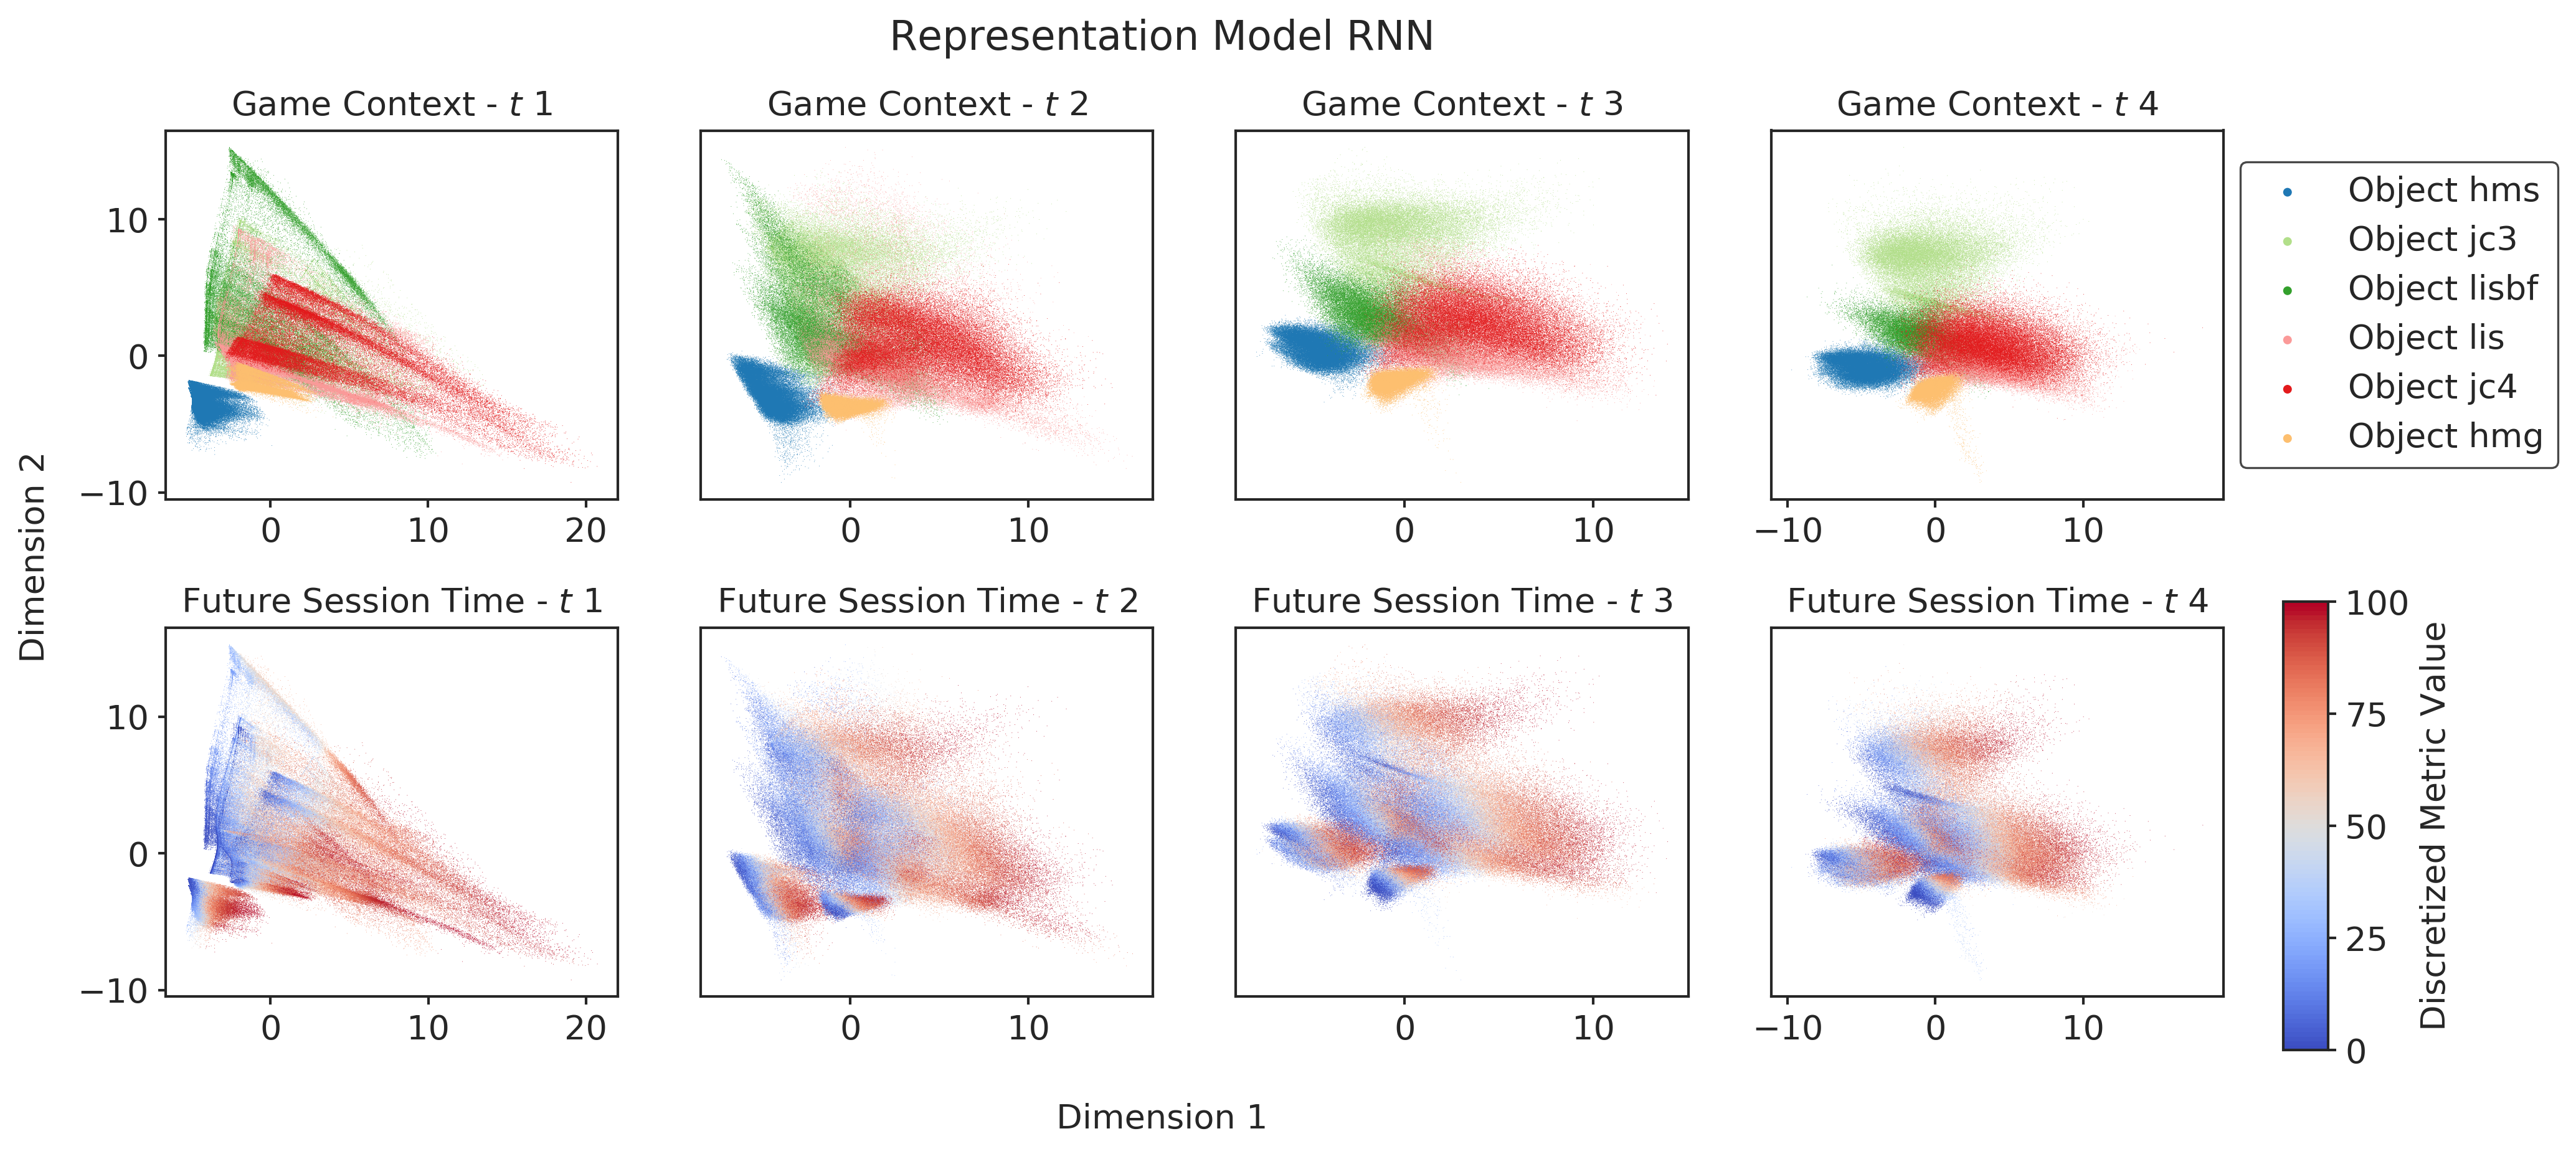
\includegraphics[width=\textwidth]{images/chapter_4/rnn_future_sess_pca.png}
\caption[\textbf{Lower dimensional representation of the latent state generated by the RNN architecture using PCA}]{The figure shows the two-dimensional projection, produced by PCA, of the multi-dimensional representation inferred by the RNN for interactions going from $t1$ to $t4$. We can read the values of the x and y axes as the first two directions of maximum variation in the latent representation. Each point indicates the representation inferred by the RNN model after observing one game session from a single user. The colours in the first row indicate the game object from which the representation is coming. Colours in the second row represent the discounted sum of all future predictions for a particular target (for example, estimated Future Session Time) $\widehat{B}_{t2:T}$ which is given by $\sum_{i=0}^{t2:T} \gamma^i\widehat{B_i}$ with $\gamma=0.1$ as illustrated in the TD Learning equation \ref{td_v}}
\label{temporal_panel_rnn_pca}
\end{figure}

we can see that the representation seems to embed a single gradient line able to distinguish individuals based on the expected length of their future interactions (here future session time) with the considered game objects. However, the low dimensional projection appears to be organized in a disorderly manner, with game contexts blending into each other causing the gradient line to look discontinuous. 

The projection produced by the UMAP algorithm, on the other side, appears to provide a better picture of the inherent structure of the inferred representation. Looking at Figure \ref{full_panel_static}A 

\begin{figure}[!htb]
\centering
\includegraphics[width=\textwidth]{images/chapter_4/static_repr_42.png}
\caption[\textbf{Lower dimensional representation of the latent state generated by the RNN architecture}]{The representation generated by the RNN model distinguishes between different game objects while maintaining an overarching organization able to capture variations in the expected intensity of future interactions that individuals will have with a specific game object. Panel A shows the two-dimensional projection, produced by UMAP, of the multi-dimensional representation inferred by the RNN at $\mathbf{t1}$ as produced by UMAP. We can read the values of the x and y axes as a coordinate system where proximity represents similarity between points in the original high-dimensional space. Each point indicates the representation inferred by the RNN model after observing one game session from a single user. The colours in the Game Context panel indicate the game object from which the representation is coming. Colours in the small panels represent the discounted sum of all future predictions for a particular target (for example, estimated Future Session Time) $\widehat{B}_{t2:T}$ which is given by $\sum_{i=0}^{t2:T} \gamma^i\widehat{B_i}$ with $\gamma=0.1$ as illustrated in equation \ref{td_v}. Each unit  encodes the intensity of future interactions through multiple non-monotonic functions. Panels B and C show the relationship between the activation of randomly-selected hidden units in the LSTM layer of the RNN and the model's predictions at $\mathbf{t1}$. Panel B shows the relationship between the discretized activation of 10 randomly selected units (artificial neurons) plotted along the y axis and the predictions made by the model at $t1$ (colour coded from blue to red as in the small panels in A) for the game object $hmg$. Panel C shows in more detail the relationship between discretized activation and RNN predictions for a single unit highlighted by a black box in Panel B. Here the x axis indicates the discretized activation while the y axis the mean discretized discounted sum of all future predictions produced by the model. Vertical lines are standard errors of the mean. The red curve is the line of best fit provided by a generalized additive model \cite{serven2018} while the box reports the MIC and the correlation coefficient (Spearman's $\rho$) between the artificial neuron activation and the model's predictions.}
\label{full_panel_static}
\end{figure}

we observe how the model was able to effectively distinguish between different game objects while simultaneously encoding for variations in the expected intensity of future interactions. This is illustrated by the fact that each game object occupies different and distinct regions in the representation space while showing a within-object gradient-like organization that places individuals (i.e. single dots) on a continuum based on the estimated magnitude of their future behaviour. 

This organization is preserved for each of the six targets showing how the representation inferred by the model is a suitable meta-descriptor for different behavioural indicators. As expected, some targets show a very similar but not identical organization (e.g. Future Session Time and Future Session Activity) while others appear to be independent (e.g. Future Session Time and Future Absence). We note that the absolute location of each game aggregate (i.e. all the points belonging to a specific game object) on the 2D plane is arbitrary. 

Panels \ref{full_panel_static}B and \ref{full_panel_static}C provide more insight into the activation profiles of individual hidden units constituting the generated representation. Panel \ref{full_panel_static}B shows the relationship between the activity of 10 randomly-chosen units and the predictions generated for the five targets. These are essentially transducer functions illustrating how the estimate for a particular target varies (on average) as the output of a units increases or decreases. Each unit seems to encode for multiple non-monotonic functions, one for each of the considered targets. Differences in the shape of these functions reflect similarities between their associated targets. For example, the functions associated to two highly related targets like Future Session Time and Future Session Activity (see panel \ref{full_panel_static}A) appear to be very similar in shape (see panels \ref{full_panel_static}B and \ref{full_panel_static}C). Interestingly, although most units appear to encode for unique functions some of them (e.g. 41 and 44) show an almost identical behaviour. This suggests the presence of redundancy in the functions underlying the representation generated by the RNN model. These observations are clarified in panel \ref{full_panel_static}C, where the functions associated with a single unit (20, indicated by a dark box in \ref{full_panel_static}B) are presented. Here we observe a strong, non-linear relationship between the unit's activity and the estimated targets (see the high MIC values and the line of best fit). In addition, the between-targets variation in MIC values suggest how the chosen unit is not equally informative for all targets but rather shows specialized  behaviour.

\begin{figure}[!htb]
\centering
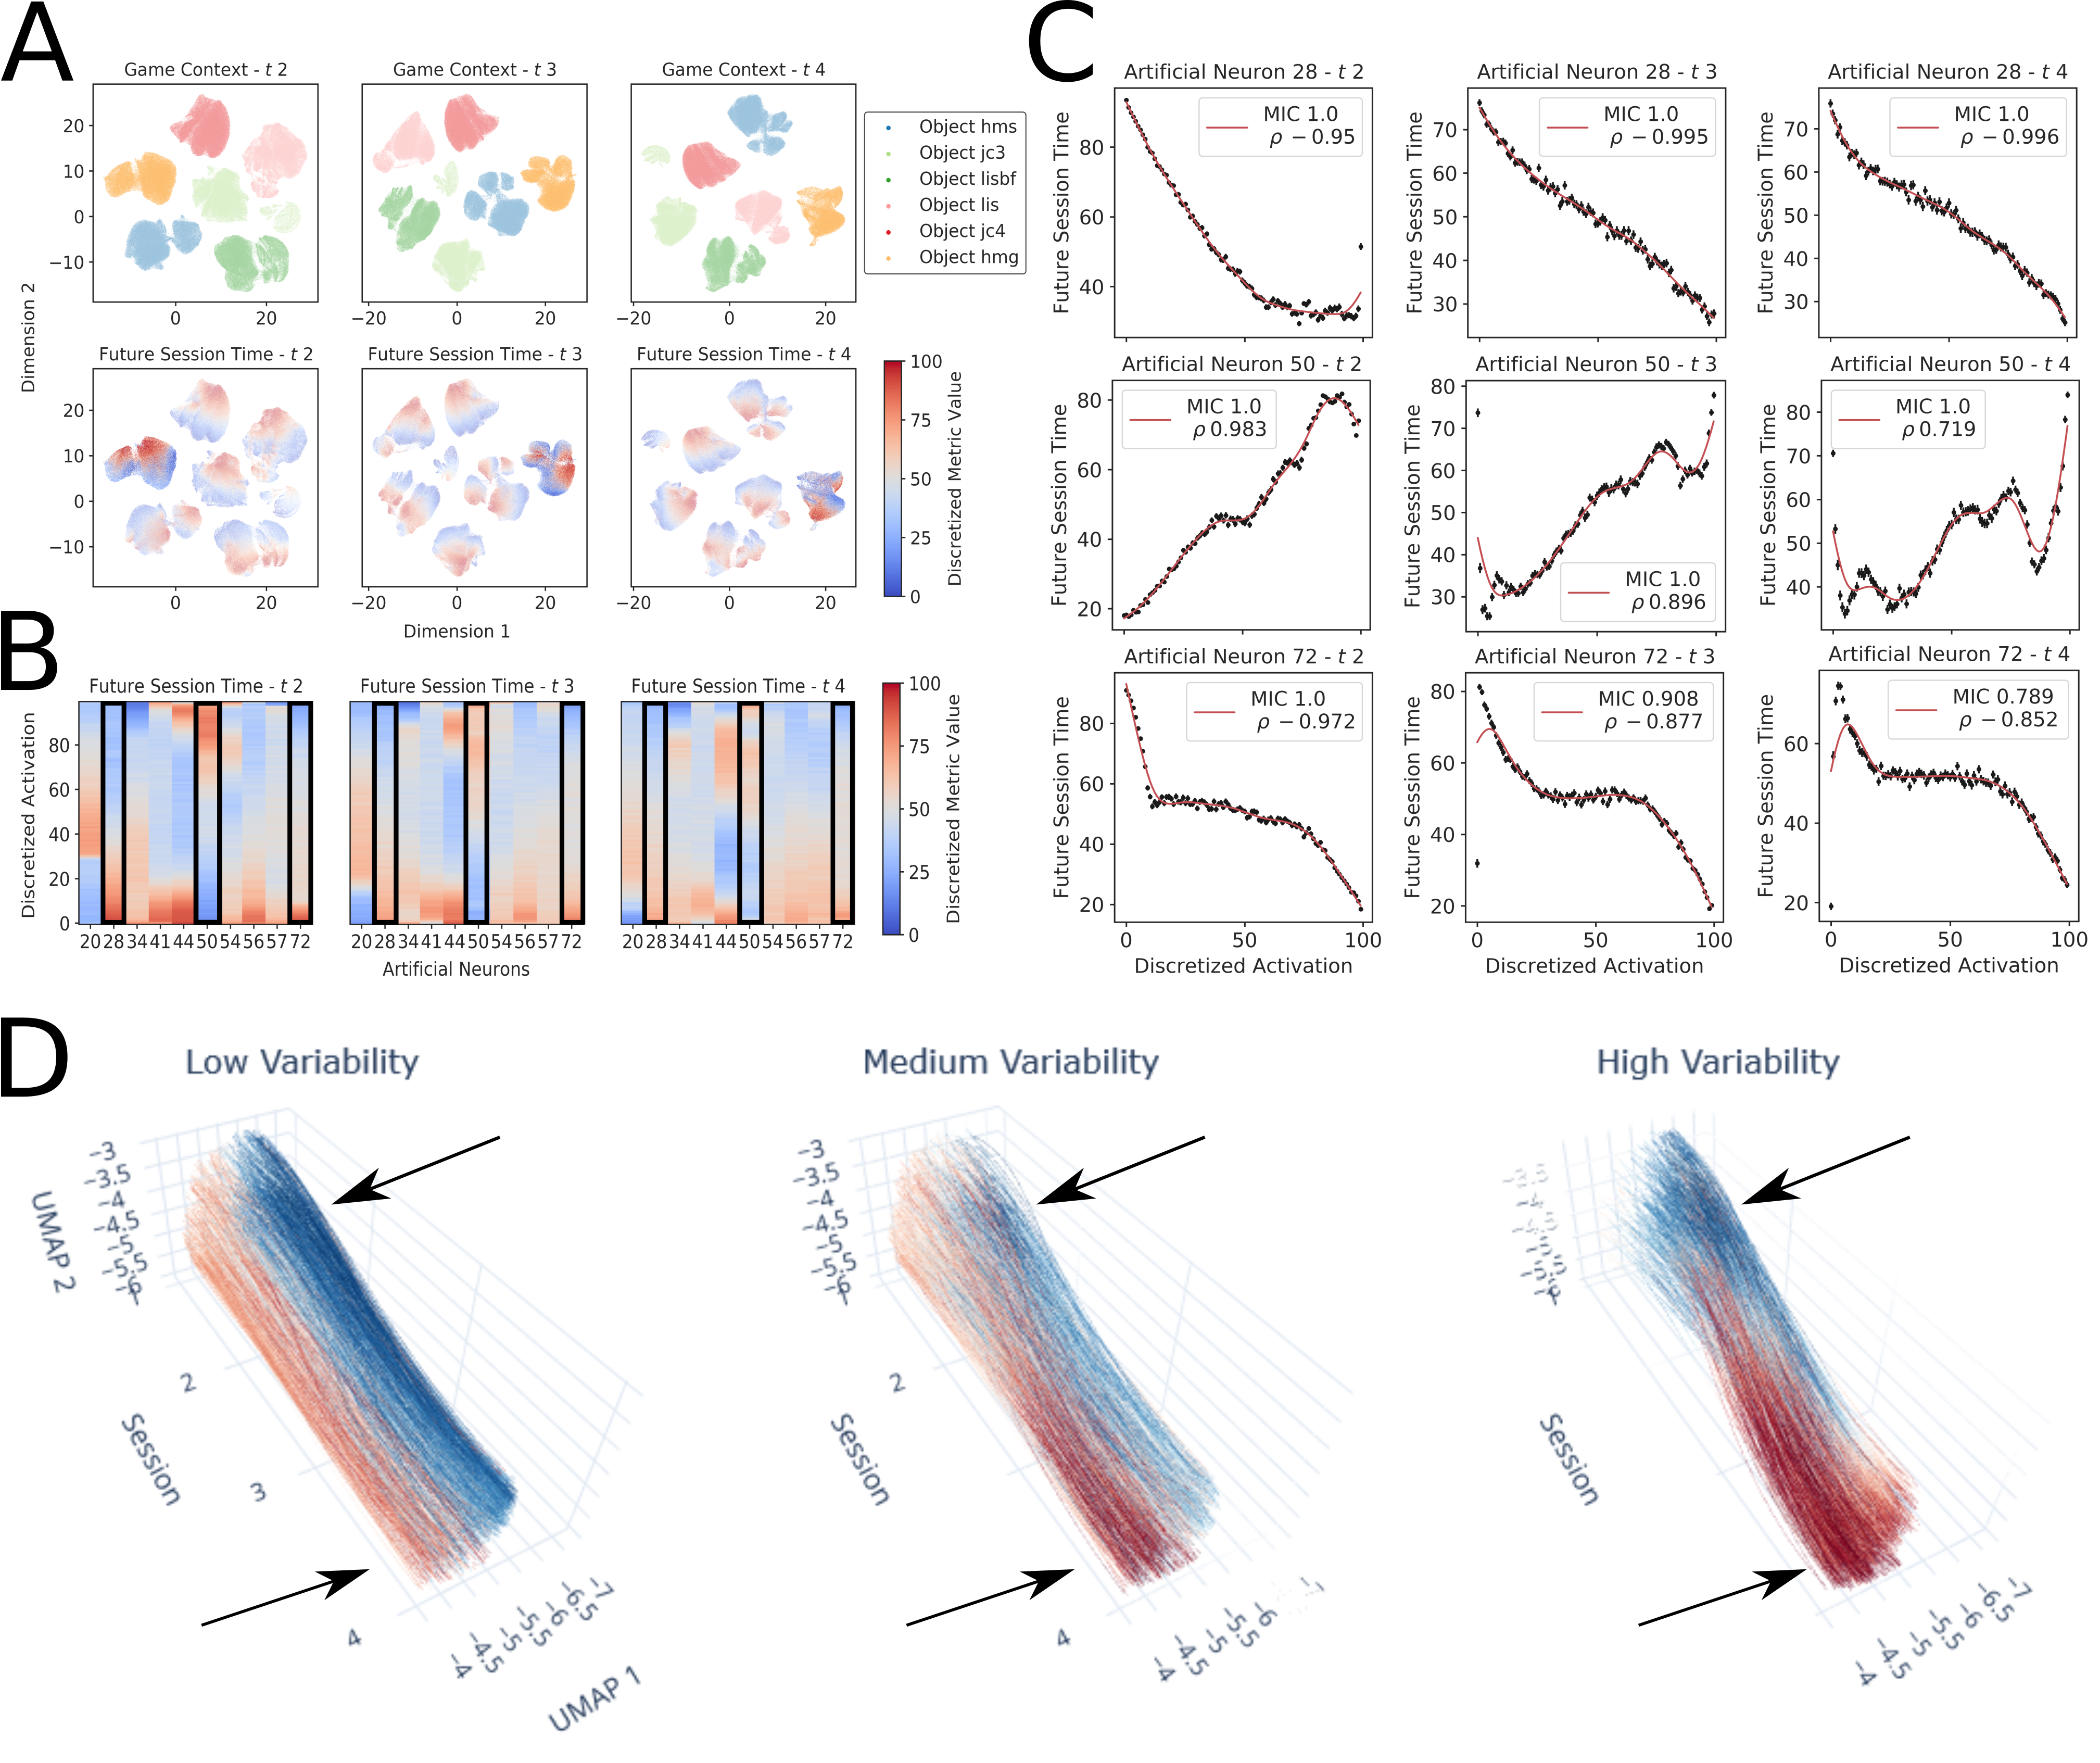
\includegraphics[width=\textwidth]{images/chapter_4/dynamic_repr_42.png}
\caption[\textbf{Lower dimensional representation of the evolution of the latent states generated by the RNN architecture}]{The representation generated by the RNN model appears to maintain its discriminant properties over time. Panel A shows a two-dimensional projection of the multi-dimensional representation inferred by the RNN at $t2$, $t3$ and $t4$. The inferred representation maintains its gradient-like organization over time with an increased ability to differentiate between game objects. As in Figure \ref{full_panel_static}, x and y axes are dimensions individuated by the UMAP algorithm and can be interpreted as a coordinate system where proximity represents similarity between points. Colours in the first row indicate which game object the representation is coming from while those in the second row indicate the discounted sum of future predictions for a single target (i.e. "Future Session Time"). \textbf{The units constituting the generated representation encode for functions that are consistent over time.} Panels B and C show the relationship between units' activation and the model's predictions over time for the game object $hmg$. Different units appear to encode the same target with different non non-monotonic functions which are relatively consistent over time. Panel B illustrates the relationship between the same 10 randomly selected units specified in figure \ref{full_panel_static} and the predictions made by the model for Future Session Time at $t2$, $t3$ and $t4$. Panel C shows in more detail the relationship of the three artificial neurons, highlighted by black boxes in B, across time. Each row is a different unit while each column corresponds to a different $t$. The x axis indicates the discretized activation while the y axis the mean discretized discounted sum of all future predictions. Vertical lines are standard errors of the mean. The red curve is the line of best fit provided by a generalized additive model \cite{serven2018} while the box report the MIC and the correlation coefficient (Spearman's $\rho$) between the artificial neuron activation and the model's predictions. \textbf{The generated representation produces areas of low and high expected intensity among which individuals move over time.} Panel D shows trajectories through time produced by a version of UMAP that incorporates temporal information. Data are drawn from random subsets of individuals having low, medium and high variability in their expected amount of future behaviour. The representation inferred by the RNN model produces "hot" (i.e. the left side) and "cold" (i.e. the right side) regions, representing high and low expected Future Session Time, that are spatially consistent over time. Individuals appear to either stay in the same region or to move between regions over time. Here each line represents variations in the representation generated by the RNN model for a single user over four temporal steps. Continuity is generated by means of cubic spline interpolation for the lines and by linear interpolation for the colours. The x and y axes are the dimensions individuated by the UMAP algorithm while the z axis indicates the associated point in time. Colours indicate the discounted sum of future predictions produced by the model at a specific point in time.}
\label{full_panel_temporal}
\end{figure}

The analyses in Figure \ref{full_panel_static} were performed at a single time point $t1$. However, as we mentioned before, the characteristics of our architectures allowed us to also evaluate how the latent representation evolved over time. 

Looking at Figure \ref{full_panel_temporal}, we can see that the characteristics detected at a single point in time remain qualitatively consistent over time. For example, focusing on Future Session Time (see Appendix \ref{rnn_architecture_representations} for results connected to other targets), we see in Figure \ref{full_panel_temporal}A that the model's ability to segregate different game objects while providing an  overarching representation of the intensity of future interactions is preserved over time. This supports the hypothesis that the representation inferred by our model is dynamic in nature which is further corroborated by panel \ref{full_panel_temporal}D. There we can see how the RNN model was able to individuate a "space" with temporally consistent ”hot” and ”cold” regions between which individuals gradually moved over time depending on the expected intensity of their future interactions. This means that given the history of interaction of a particular individual with a specific game object, our model would determine their "position" (i.e. their "internal state") in a latent space indicative of the expected intensity of future interactions with that object. If we recall our definition of attributed incentive salience from chapters \ref{chapter_lit_review} and \ref{chapter_theory_modelling} we can suggest that the model has inferred the location of individuals in what is an approximation (from the functional point of view) of the "attributed incentive salience space". This aligns with the manifold hypothesis mentioned in sections \ref{manifold_rep_incentive_salience} and \ref{manifold_learning}: changes in the propensity to interact with a specific game object (i.e. variations in the amount of attributed incentive salience) can be expressed moving on a manifold embedded within an $h$ dimensional space, with $h$ being the dimensionality of the representation generated by our RNN model. 

It appears that the hidden units constituting this representation tend to be consistent over time in the type of functions they encode (see Figure \ref{full_panel_temporal}B and C). As expected, we can again observe a strong non linear association between units' activation and targets' predictions, see MIC values and lines of best fit. The decrease in MIC value observed in Figure \ref{full_panel_temporal}C for the artificial neuron 72 might indicate how certain units lose their informative power over time.

\begin{figure}[!htb]
\centering
\includegraphics[width=\textwidth]{images/chapter_4/RNN_MLP_repr_42.png}
\caption[Lower dimensional representation of the latent states generated by the time-distributed MLP architecture]{The representation generated by the MLP model is less effective at distinguishing between different game objects and different levels of expected future behaviour intensity. Panel A shows a two-dimensional projection of the multi-dimensional representation inferred by the MLP at $t1$, $t2$, $t3$ and $t4$. Differently from the RNN, the representation shows a disruption in the gradient-like organization and a reduced ability to differentiate between game objects which remain constant over time. The x and y axes are dimensions individuated by the UMAP algorithm and can be interpreted as a coordinate system where proximity represents similarity between points. Colours in the first row indicate which game object the representation is coming from while those in the second row indicate the discounted sum of future predictions for a single target (i.e. "Future N° of Sessions") \textbf{The representation generated by the MLP model is less effective at at distinguishing different levels of expected behaviour intensity for states that are further away in the future.} Panel B shows a two-dimensional projection of the multi-dimensional representation inferred by the RNN (left) and MLP(right) at $t1$ but colour coded with the discounted sum of future predictions from $t4$ onward. The representation generated by the RNN is able to maintain a gradient-like organization even from states that are further away in the future while this capacity is almost entirely lost for the MLP. The colours in the Game Context panel indicate the game object from which the representation is coming. Colours in the small panels represent the discounted sum of all future predictions for a particular target computed from $t4$ onward instead that from $t1$. The x and y axes are the dimensions individuated by the UMAP algorithm.}
\label{predictive_panel}
\end{figure}

If we look at the differences between MLP and RNN-like architectures from section \ref{model_architecture_2}, we can see that they all aim to solve the same task: predict the intensity of future behaviour given the history of interactions. They do so relying on the same type of metrics, leveraging similar computational mechanisms (i.e. multitask learning and non-linearity) and producing representation according to the same underlying principle (i.e. the manifold hypothesis). Nevertheless, the fact that MLP architectures consistently provided poorer fit to data already suggests that whatever representation it had inferred it was likely a sub-optimal approximation of the manifold structure of attributed incentive salience. 

Looking at figure \ref{predictive_panel}A, and knowing that UMAP represents differences and similarities between points through distance, we can see how the representation generated by the MLP less clearly differentiate between game objects. On the same figure, we can notice how the gradient representation for the metric Future N° Sessions is largely disrupted. This effect is however consistently less pronounced for other metrics (see Appendix \ref{mlp_architecture_representations} for additional visualizations) and in accordance to the differences in predictive perfromance that we observed in chapter \ref{chapter_implementation_testing}. 

Recalling what mentioned in section \ref{comp_framework}, the latent state produced by the level of attributed incentive salience should retain at any point in time some predictive power over the intensity of all the future interactions (i.e. not just the one that follows). Figure \ref{predictive_panel}B shows the representation generated by RNN and MLP at $t1$ but color coded with the discounted sum of the predictions made from $t4$ onward. We can see that, even if degraded, RNN still preserves some of the desired gradient-like organization which is instead much more disrupted for MLP. This is in accordance to what is shown by Figure \ref{full_panel_temporal}D: the RNN appears to define regions of high and low expected behavioural intensity which are consistent over time rather than generating representations that are mostly representative of what is expected at $t+1$.

\subsection{Evaluating the Contribution of Environmental and Game Events Covariates}
\label{representation_env_even_contr}
Shifting our attention to the representations generated by the improved version of the RNN architecture we can see some noticeable differences. Looking at Figure \ref{rnn_env_even_full_beha} 

\begin{figure}[!htb]
\centering
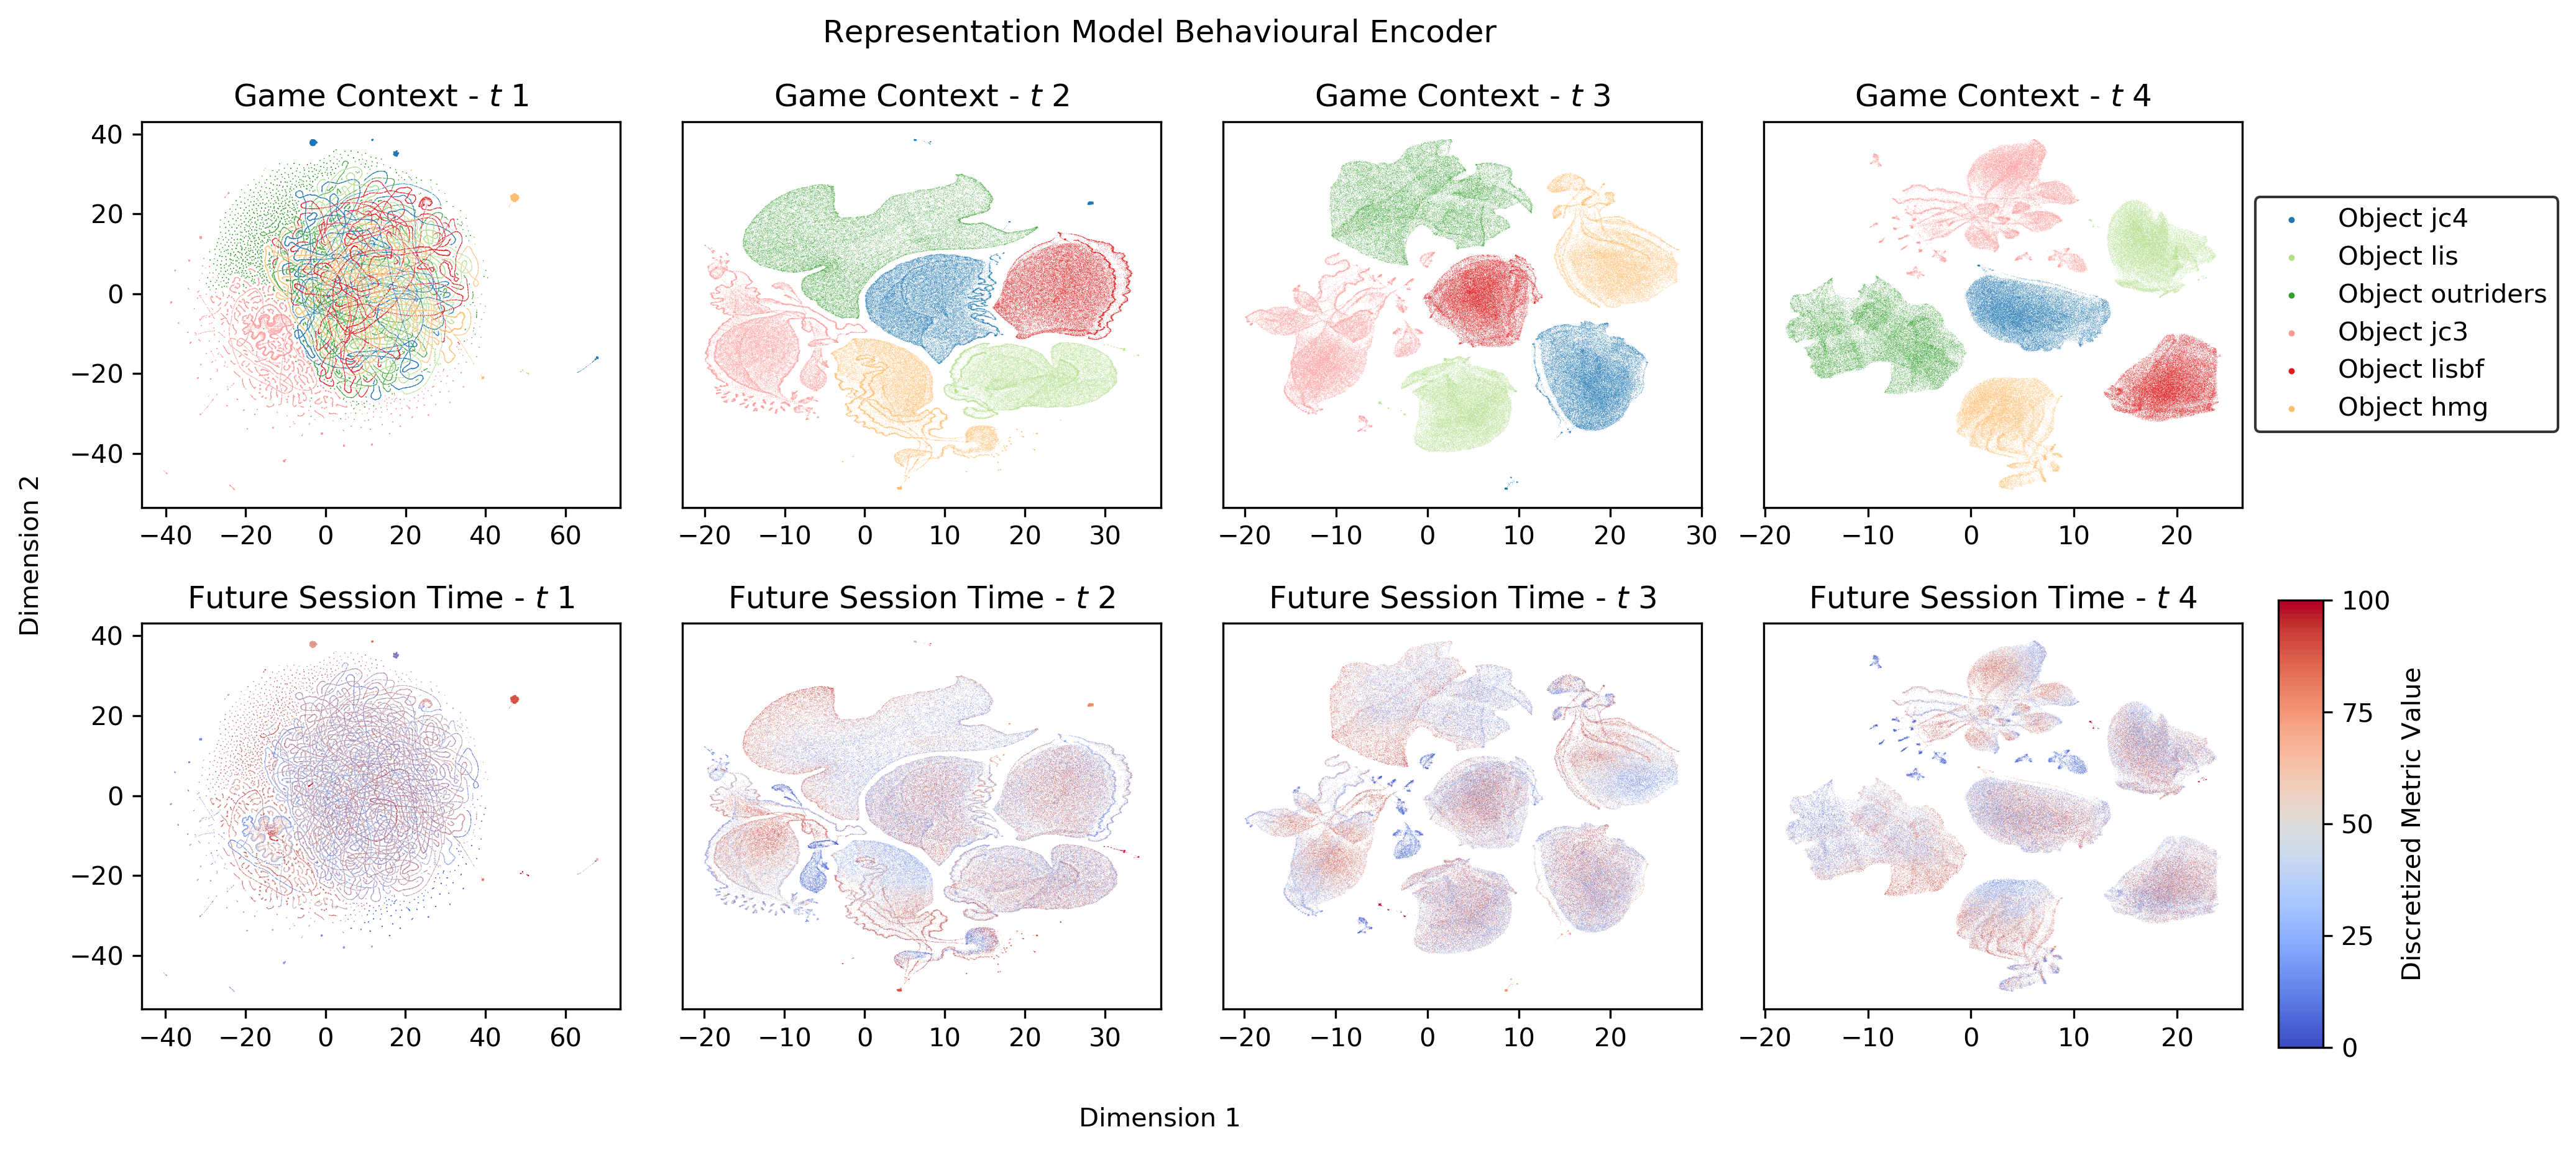
\includegraphics[width=\textwidth]{images/chapter_4/RNN_env_even_0_lstm_layer_features_Future Session Time.png}
\caption[\textbf{Lower dimensional representation of the latent representations generated by the improved version of the RNN architecture from the behavioural metrics}]{Each panel shows a two-dimensional projection of the multi-dimensional representation inferred by the improved RNN architecture at $t1$, $t2$, $t3$ and $t4$. The representations presented in this figure have been generated by the portion of the architecture receiving the behavioural metrics as input. As in Figure \ref{full_panel_temporal}, x and y axes are dimensions individuated by the UMAP algorithm and can be interpreted as a coordinate system where proximity represents similarity between points. Colours in the first row indicate which game object the representation is coming from while those in the second row indicate the discounted sum of future predictions for a single target (i.e. "Future Session Time").}
\label{rnn_env_even_full_beha}
\end{figure}

we can see how the representation generated from the behavioural metrics changes considerably from the simple RNN architecture. Despite the ability to differentiate between game objects is, up to a certain degree, preserved, the quality of the gradient organization is markedly diminished. This is doesn't come as a surprising result: similarly to what happens when covariates are added in a linear model, the behavioural metrics are now only one of the components making up the final representation in charge of producing the model's predictions. It is however worth noticing that the ability to differentiate between individuals with respect to the intensity of their future interactions is not completely removed suggesting the intensity of past interactions still plays a role in determining the intensity of future ones. 

The same cannot be said for the representation generated by the environmental metrics. If we look at Figure \ref{rnn_env_even_full_env} we can see that not just the ability to differentiate between game objects is almost completely disrupted, but also the capacity to distinguish between individuals with high and low expected intensity of future interactions. 

\begin{figure}[!htb]
\centering
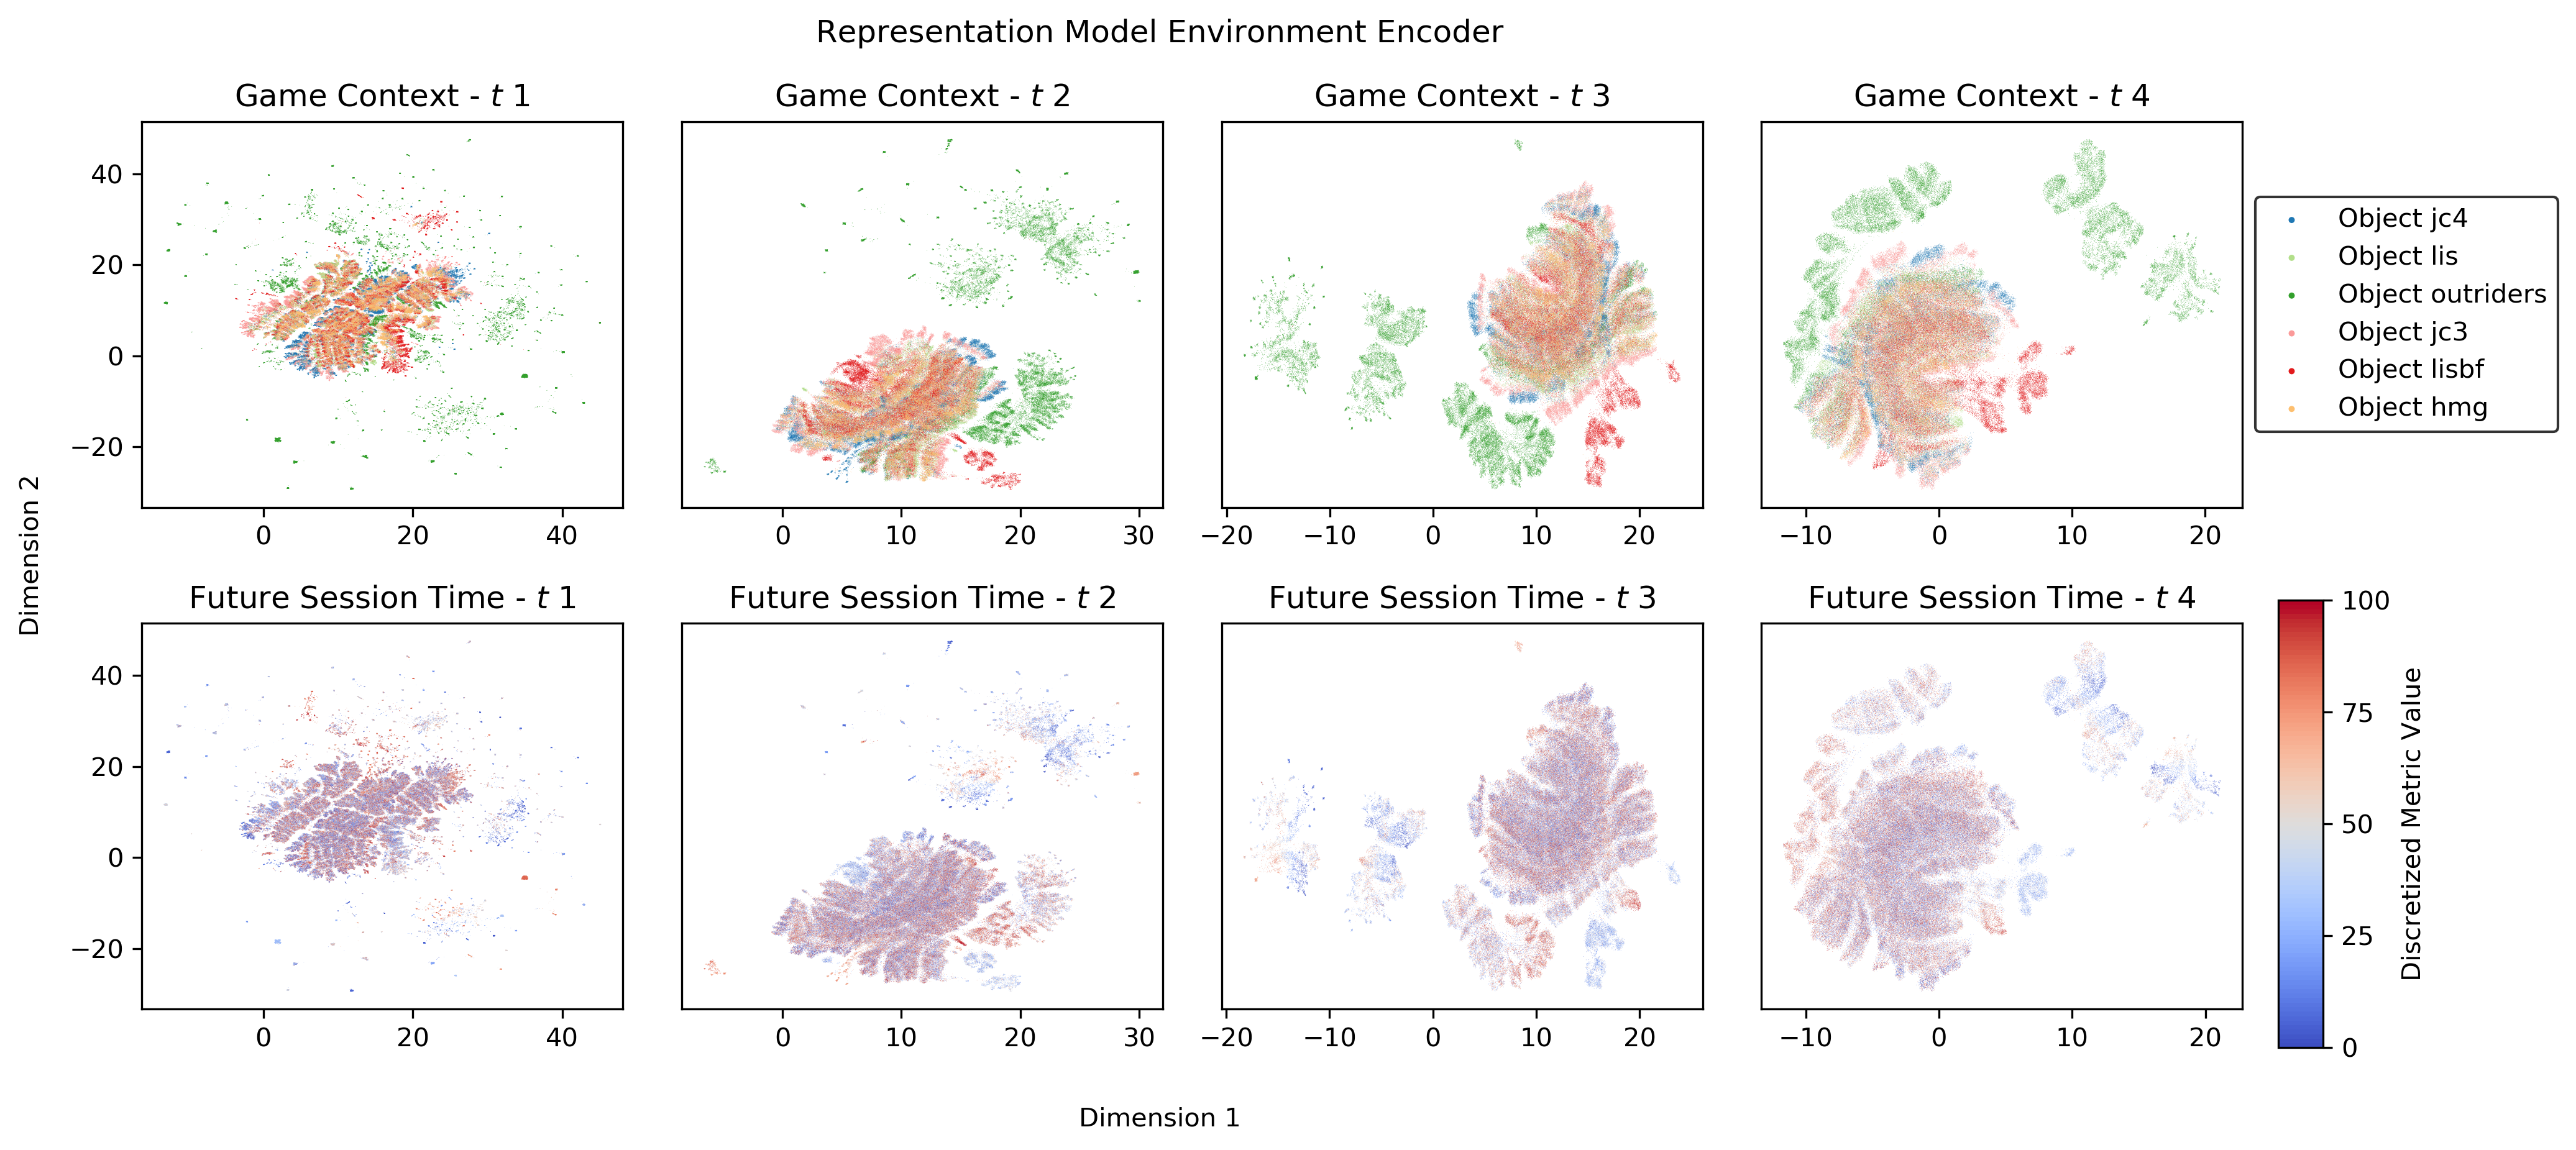
\includegraphics[width=\textwidth]{images/chapter_4/RNN_env_even_0_lstm_layer_env_Future Session Time.png}
\caption[\textbf{Lower dimensional representation of the latent representations generated by the improved version of the RNN architecture from the environmental metrics}]{Each panel show a two-dimensional projection of the multi-dimensional representation inferred by the improved RNN architecture at $t1$, $t2$, $t3$ and $t4$. The representation presented in this figure has been generated by the portion of the architecture receiving the environmental metrics as input. As in Figure \ref{full_panel_temporal}, x and y axes are dimensions individuated by the UMAP algorithm and can be interpreted as a coordinate system where proximity represents similarity between points. Colours in the first row indicate which game object the representation is coming from while those in the second row indicate the discounted sum of future predictions for a single target (i.e. "Future Session Time").}
\label{rnn_env_even_full_env}
\end{figure}

As we anticipated in sections \ref{model_architecture_3} and \ref{modelling_env_and_game_elements}, we did not expect the environmental variables to have strong predictive power on future ammount of gaming behaviour, but rather to act as an absorbing factor for possible noise observed in the behavioural metrics. Or better, we argued that environmental factors might affect the behavioural manifestations of a certain latent state (i.e. attributed incentive salience) both in the past and in the future, but do not play a central role in the shaping of the state itself (i.e. the level of attributed incentive salience). We will expand more on this section \ref{partition_environment}).

Another possibility is that the environmental information do not play a relevant role in generating a latent representation with good predictive power and are just treated as noise by the model. However, by looking at the occasional improvements in predictive performance that they provided in section \ref{results_3}, it seems more plausible that they are to be considered as nuisance metrics supporting the role of the other model inputs. 

In spark contrast with the previous two representations is the one generated from the game events information. Looking at Figure \ref{rnn_env_even_full_events} we can see how differently from what we observed in Figure \ref{rnn_env_even_full_beha} the representation appears highly fragmented but with each fragment consistently belonging to distinct game contexts. This suggests the representation attempted to encode the heterogeneity in sequences of game events while maintaining them within the same context.

\begin{figure}[!htb]
\centering
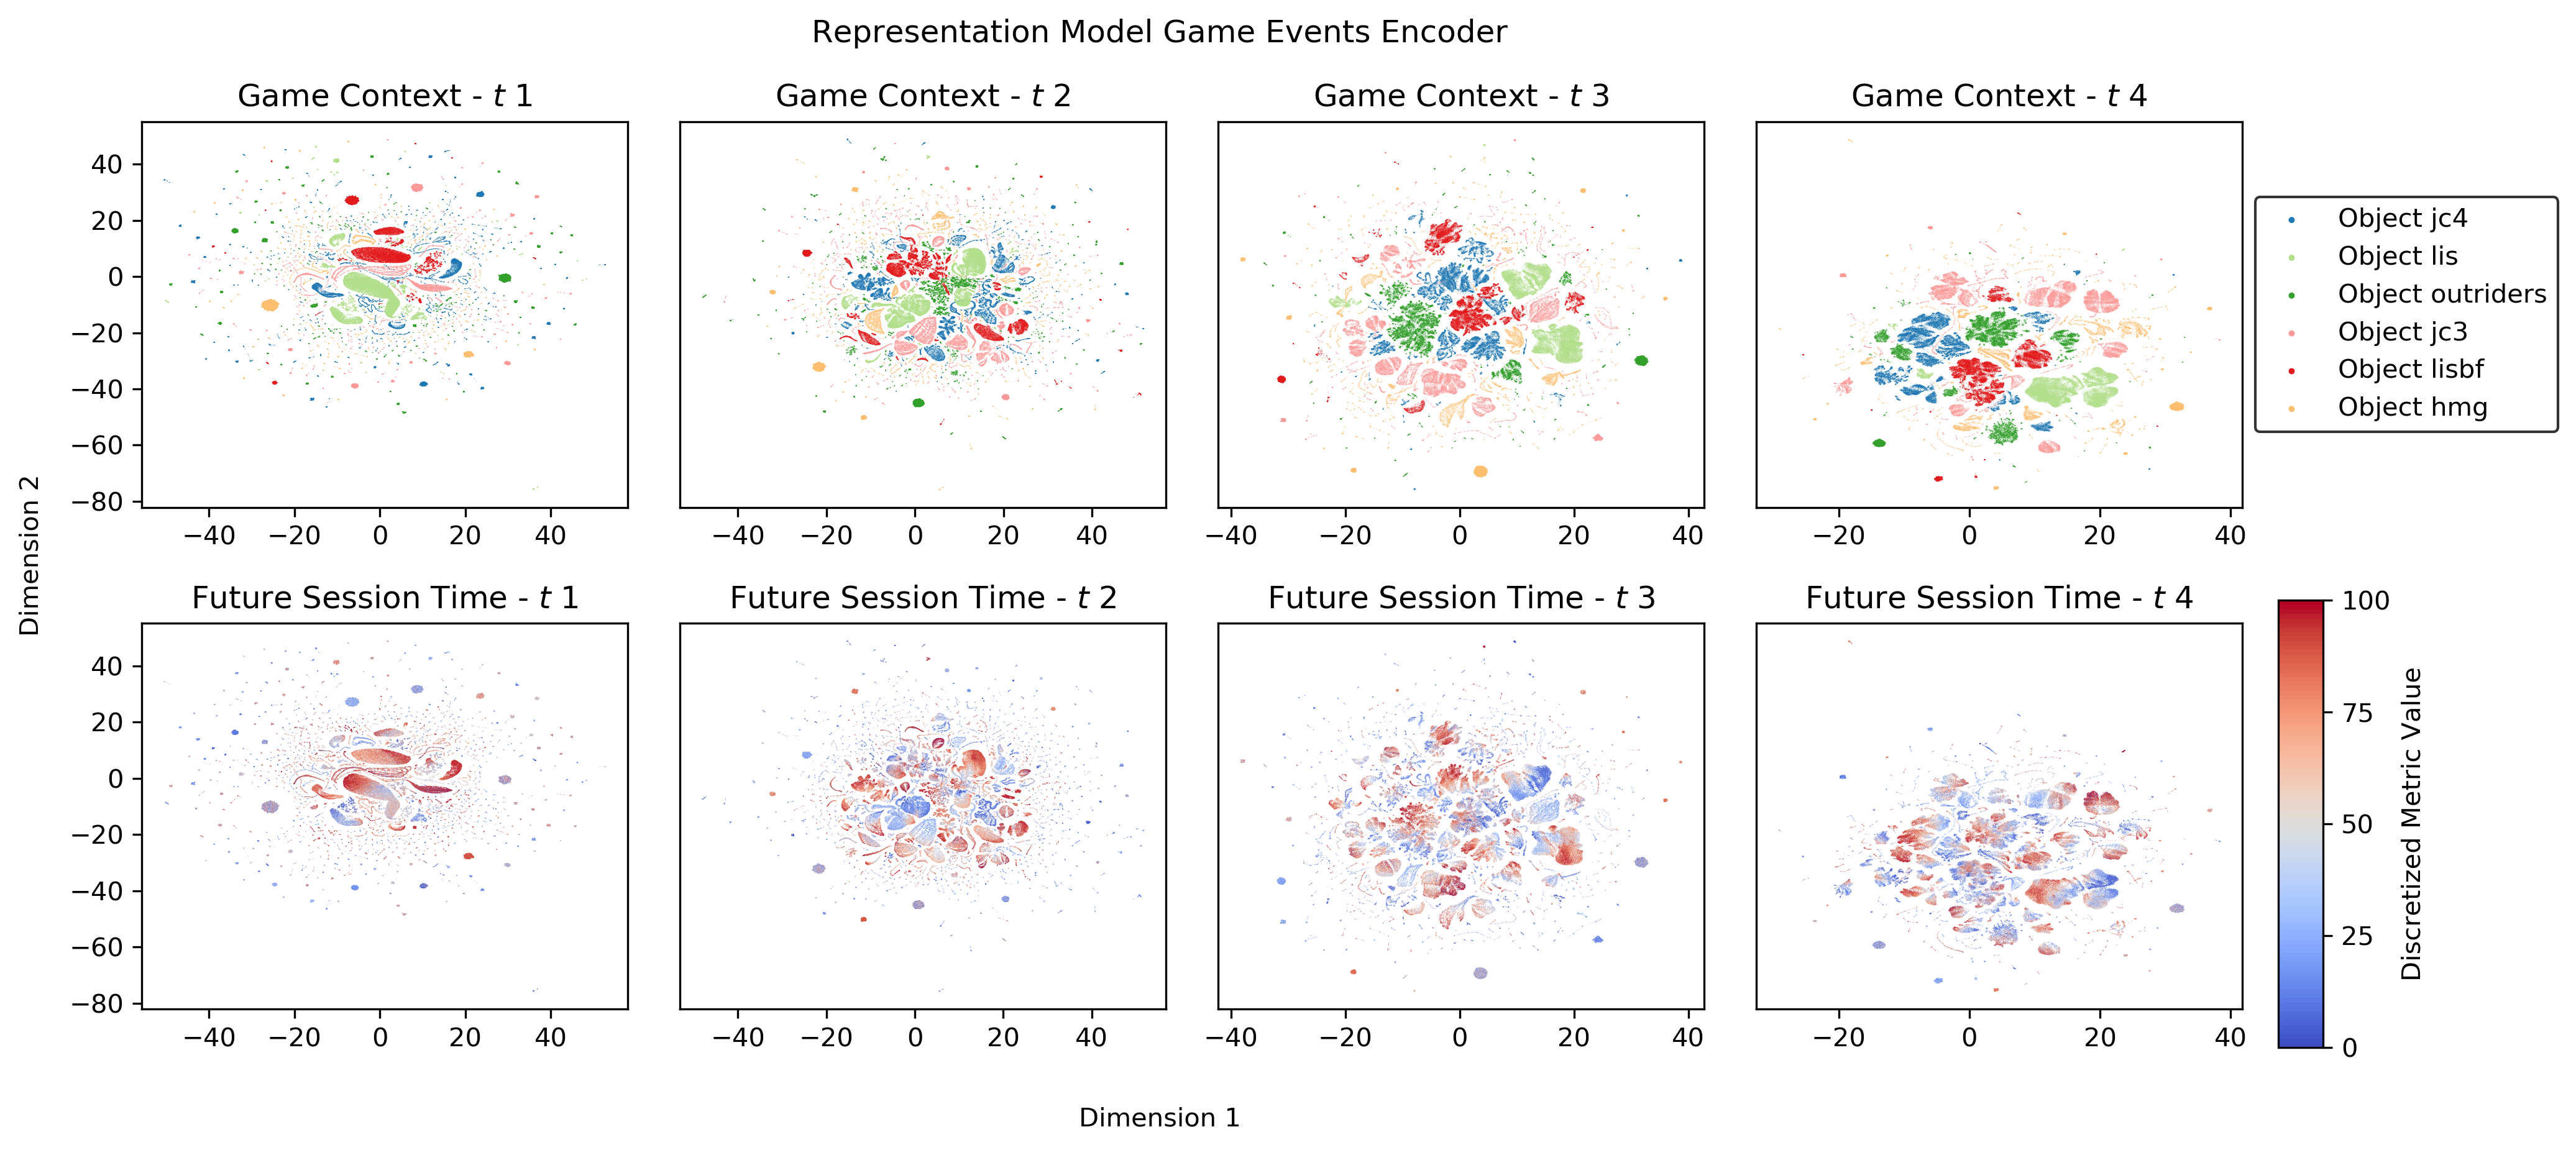
\includegraphics[width=\textwidth]{images/chapter_4/RNN_env_even_0_lstm_layer_events_Future Session Time.png}
\caption[\textbf{Lower dimensional representation of the latent representations generated by the improved version of the RNN architecture from the game events metrics}]{Each panel show a two-dimensional projection of the multi-dimensional representation inferred by the improved RNN architecture at $t1$, $t2$, $t3$ and $t4$. The representation presented in this figure has been generated by the portion of the architecture receiving the game events metrics as input. As in Figure \ref{full_panel_temporal}, x and y axes are dimensions individuated by the UMAP algorithm and can be interpreted as a coordinate system where proximity represents similarity between points. Colours in the first row indicate which game object the representation is coming from while those in the second row indicate the discounted sum of future predictions for a single target (i.e. "Future Session Time").}
\label{rnn_env_even_full_events}
\end{figure}

The observed level of fragmentation is in line with all the possible sets arising by the combination of the considered game events and their relative frequency of interactions. For example considering the tuple $\{event, frequency\}$ we could have:

\begin{gather}
\label{seq_differences}
    \{\{combat, 10\}, \{explore, 3\}, \{achievement, 2\}\} \\ \nonumber
    \neq \\ \nonumber
    \{\{combat, 2\}, \{explore, 10\}, \{achievement, 5\}\} \\ \nonumber
    \neq \\ \nonumber
    \{\{dialogue, 2\}, \{puzzle, 10\}, \{achievement, 5\}\} \\ \nonumber 
    \neq \\ \nonumber
    \dots
\end{gather}

This type of behaviour is comparable to what can be observed when analyzing words embedding of different text corpuses (e.g. see the Open Syllabus project \cite{opensyllabus}) and suggest that the architecture was able to discern differences in the sequential choices made by the individuals when interacting with different in-game elements.

What is most interesting however is that among the representations inspected so far, the one generated from the game events metric is the one better preserving the gradient organization observed for the simple RNN architecture. This suggest the the sequences of observed interactions with specific in-game mechanics plays a relevant role in differentiating between individuals with respect to the expected intensity of their future interactions with a specific game object, something that we anticipated in sections \ref{factors_engagement} and \ref{modelling_env_and_game_elements} and that is in line with previous findings in the videogame literature \cite{makarovych2018like}.

Finally, when looking at the shared representation in Figure \ref{rnn_env_even_full_shared}, we can see how it resembles the one generated by the simplified version of the RNN architecture with the only difference being a more clearly defined gradient organization. This representation is functionally equivalent to the one extracted by the simplified RNN architecture (i.e. it is used for performing multi-task learning) and is hypothesized to approximate the manifold structure of attributed incentive salience.

\begin{figure}[!htb]
\centering
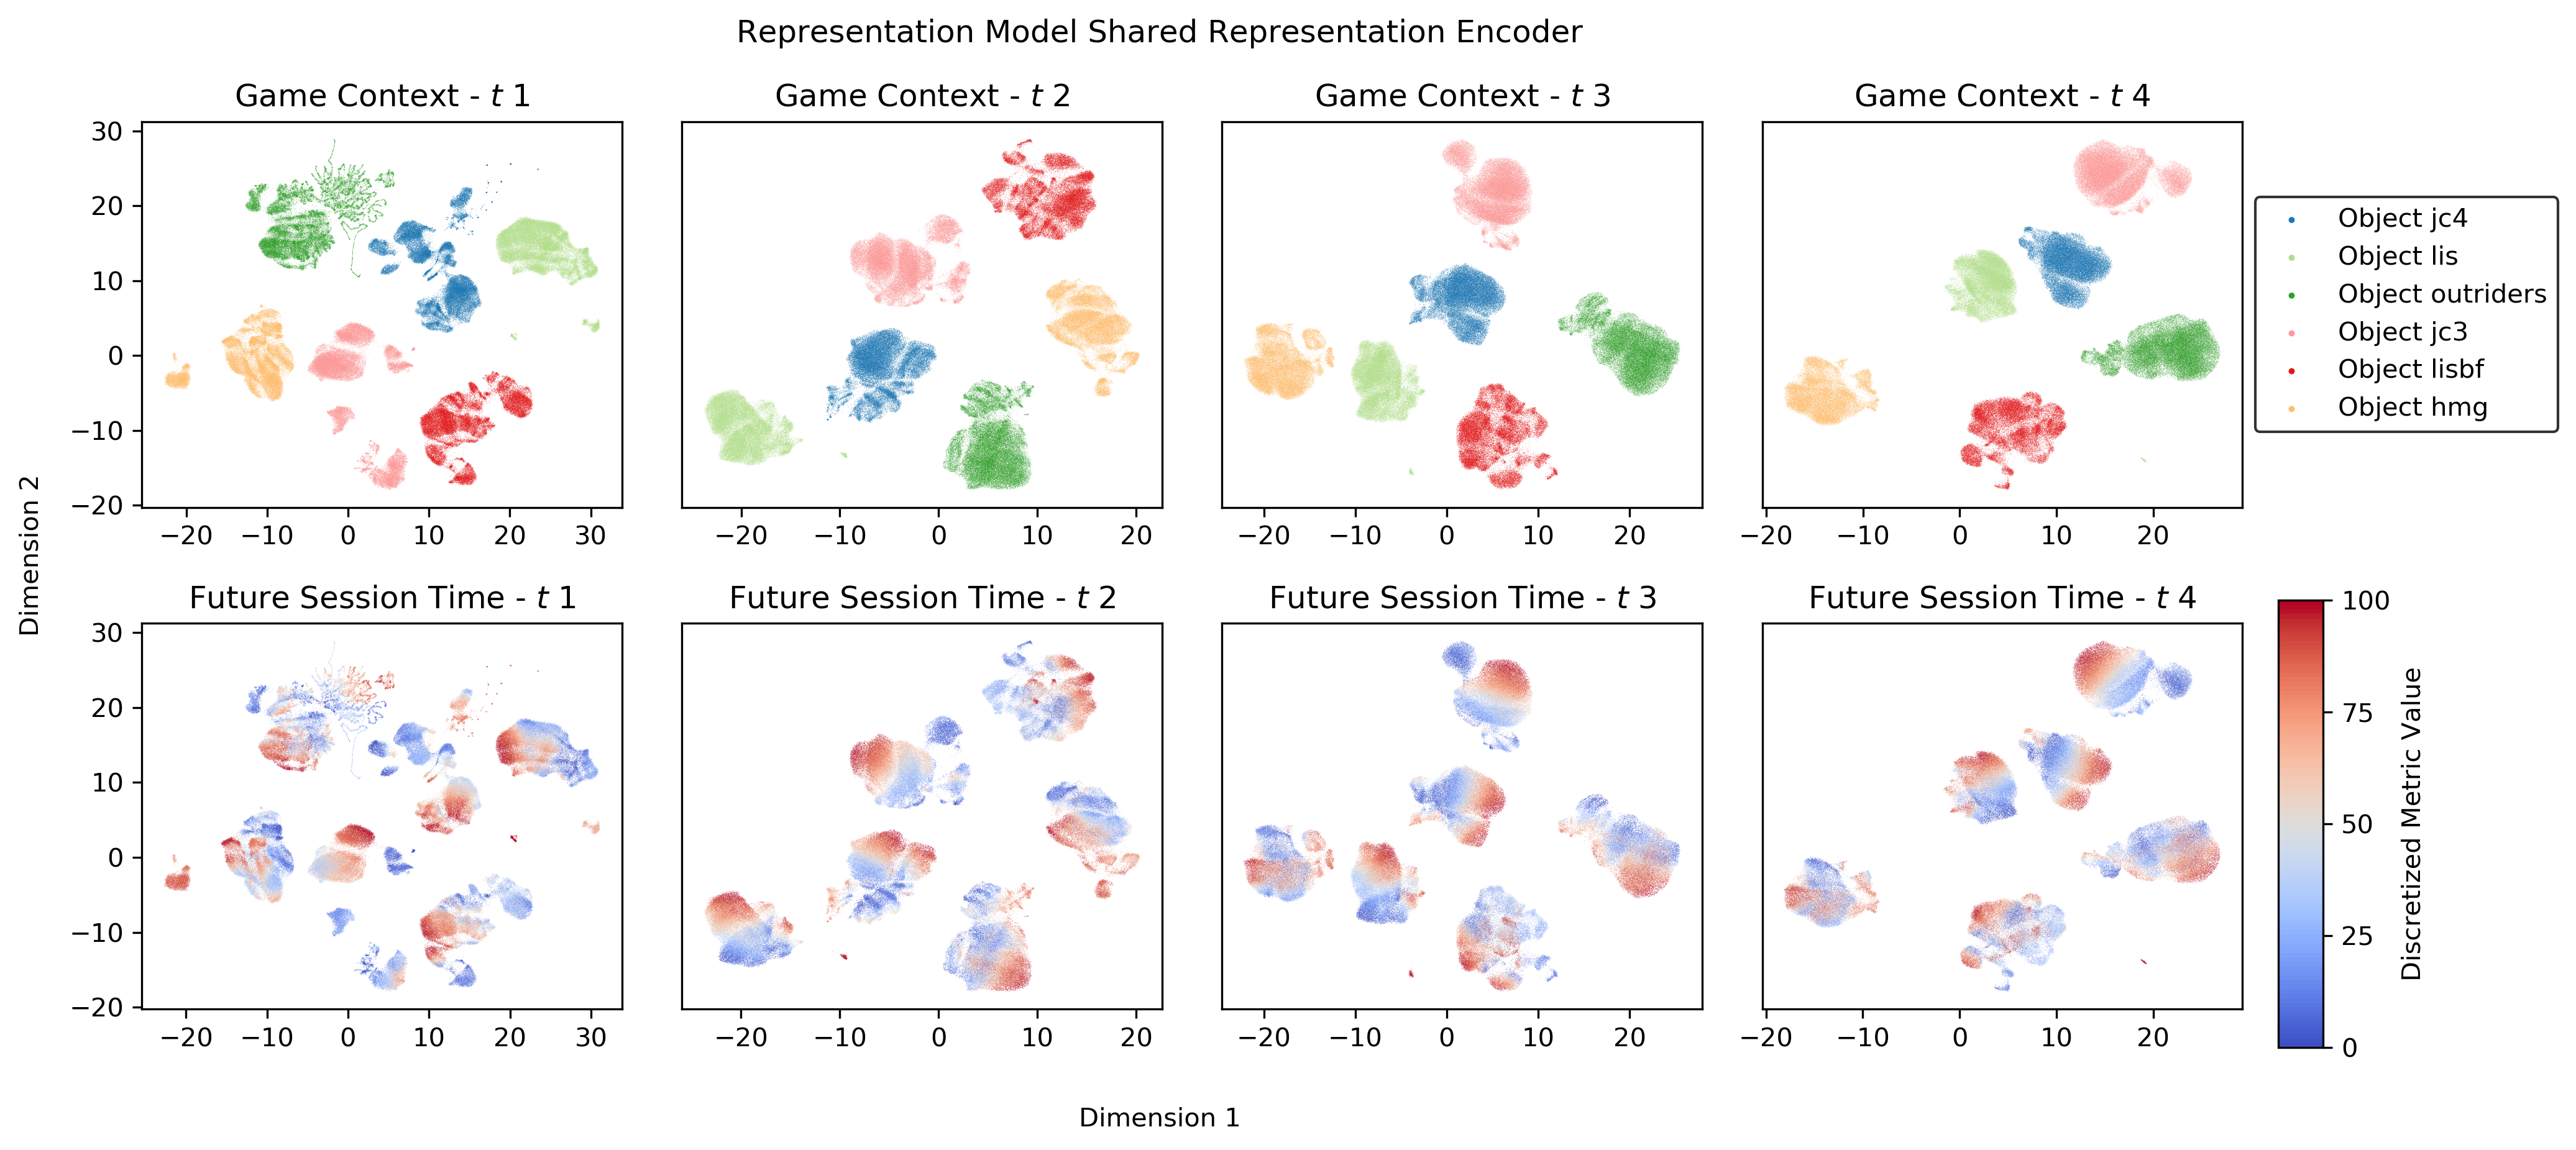
\includegraphics[width=\textwidth]{images/chapter_4/RNN_env_even_0_lstm_layer_shared_Future Session Time.png}
\caption[\textbf{Lower dimensional representation of the shared latent representations generated by the improved version of the RNN architecture}]{Each panel show a two-dimensional projection of the multi-dimensional representation inferred by the improved RNN architecture at $t1$, $t2$, $t3$ and $t4$. The representation presented in this figure has been generated by the portion of the architecture receiving as inputs the representations associated with the behavioural, environmental and game events input and is the one hypothesized to approximate the manifold structure of attributed incentive salience. As in Figure \ref{full_panel_temporal}, x and y axes are dimensions individuated by the UMAP algorithm and can be interpreted as a coordinate system where proximity represents similarity between points. Colours in the first row indicate which game object the representation is coming from while those in the second row indicate the discounted sum of future predictions for a single target (i.e. "Future Session Time").}
\label{rnn_env_even_full_shared}
\end{figure}

This qualitative improvement can be better appreciated when comparing the representation generated by the two version of the RNN architecture, color coded using the ground truth values rather than the predictions provided by the models. Looking at Figure \ref{rnn_predictive_comparison}

\begin{figure}[ht]
\centering
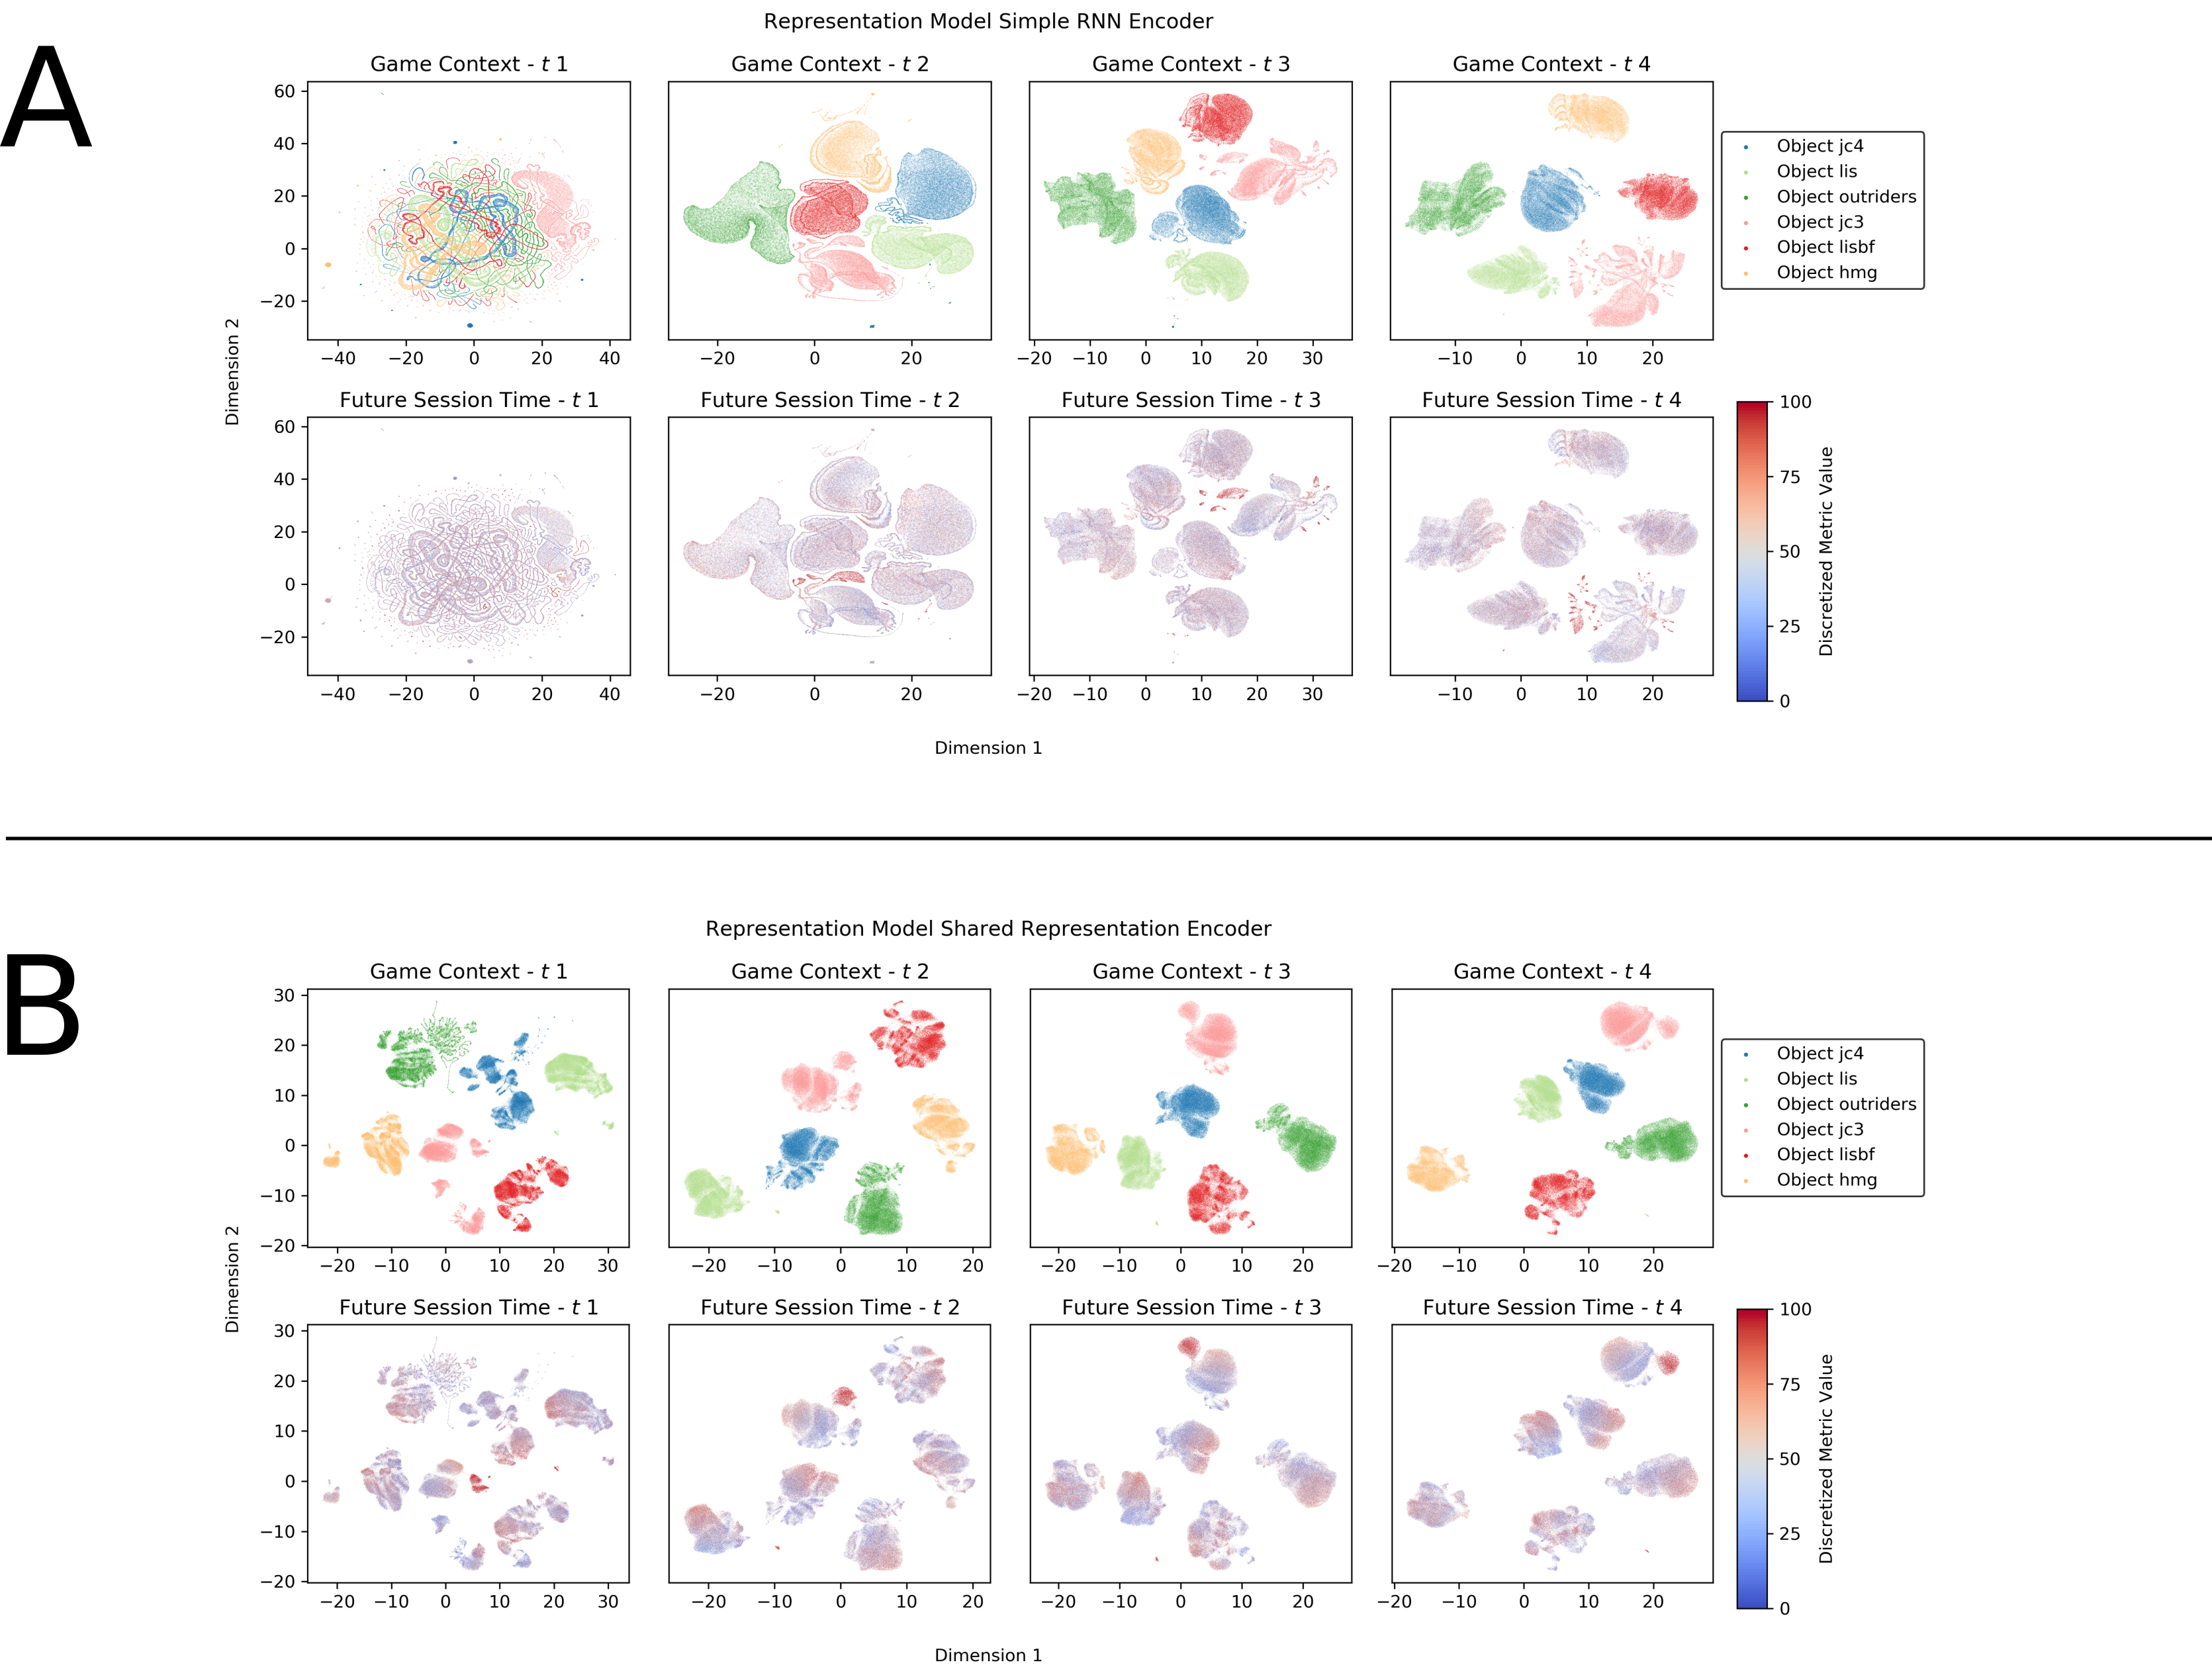
\includegraphics[width=\textwidth]{images/chapter_4/rnn_predictive.png}
\caption[\textbf{Differences in predictive power between the representations generated by the RNN architecture and its improved version}]{The figure show the two-dimensional projection, produced by UMAP, of the multi-dimensional representation generated by the RNN architecture and its improved version at $t1$, $t2$, $t3$ and $t4$. Both representations have been extracted by the portion of the architecture hypothesized to approximate the manifold structure of attributed incentive salience. Panel A refers to the RNN architecture while panel B to its improved version (including environmental and game events covariates). As in Figure \ref{full_panel_temporal}, x and y axes are dimensions individuated by the UMAP algorithm and can be interpreted as a coordinate system where proximity represents similarity between points. Colours in the first row indicate which game object the representation is coming from while those in the second row indicate the discounted sum of future ground truth values for a single target (i.e. "Future Session Time").}
\label{rnn_predictive_comparison}
\end{figure}

we can see how the simplified RNN architecture shows a greater level of disruption in the gradient like organization than its improved version, suggesting that this last one is likely better approximating the functional properties of the latent state (i.e. the level of attributed incentive salience) that generated the observed behaviour. By looking at figure \ref{rnn_env_even_full_shared}, we can notice how the topological characteristics of the previous 3 representations are replaced by the global-local organization that we described in \ref{functional_properties}. This consistency corroborates the idea that this type of organization is the most suitable one for the type of predictive task that the two architectures are aiming to solve.

\section{Partition Analysis}
\label{partition_analysese}
In order to gather additional insights on the functional properties of the representations generated by our architectures, we attempted to map what inferred by the models back to the observable behavioural space. As specified in section \ref{manifold_learning} these representations are derived from the input metrics and can be interpreted as coordinates on the manifold structure inferred by the architectures. In this view, partitioning them allows identify areas of the manifold holding information about the history of interactions between an individual and a given video game object. Moreover, since the manifold is constructed for being informative of the intensity of future interactions, different partitions might represent not just variations in the input metrics (e.g. differences in the sequences of events triggered in the game) but also in the level of attributed incentive salience. In this view, by individuating the set of metrics that contributed in defining the topology of different regions of the inferred manifold we hoped to gather insights on their role in determining the intensity of future behaviour. 

To perfrom the mapping we opted for an unsupervised approach and conducted a partition analysis on the representations extracted by the different encoders. 
To partition the data, we decided to apply Mini-Batch K-Means \cite{sculley2010web}, a variation of K-Means, to the representation extracted by the three encoders mentioned in section \ref{representation_analysis}. Given a dataset, the algorithm attempts to divide it by iteratively moving $k$ centroids so as to reduce variance within each partition. The choice of Mini-Batch K-Means was dictated by the fact that it is one of the few distance-based algorithms that scales to very large datasets. The reason for choosing a distance-based algorithm can be found in paragraph \ref{manifold_learning}, there we specified how distance in the manifold structure inferred by an ANN can be interpreted as a measure of similarity between its input with respect to the objective function that the model is trying to minimize. 

To select the optimal $k$ value, we first fitted the algorithm with a varying number of centroids (i.e. 2 to 10) and computed the associated inertia, a measure of within cluster variance (see \ref{inertia)}. Since inertia tends to zero as $k$ approaches the number of points in the dataset, we defined the optimal number of partitions as the value of $k$ at which the inertia reached its "elbow" or maximum curvature \cite{satopaa2011finding}. This allows to individuate at which number of partitions there are diminishing returns in terms of within cluster variance reduction. Despite this procedure might be prone to errors or imprecisions (e.g. the elbow might be non-unique or change depending on the maximum number of considered centroids) we thought it would be preferable to an arbitrary choice. 

Every instance of Mini-Batch K-Means was initialized 3000 times at random and ran for a maximum of 3000 epochs. The input data were re-scaled to have zero mean and unit-variance and passed to the algorithm in random batches of size $(512 \times h)$. The associated behavioural profiles were found by applying this methodology separately to each game object and retrieving for each partition the expected deviation of all the behavioural metrics from their relative mean (computed along the temporal dimension) in each game context. In order to have an indication of the quality of the individuated partitions, we decided to compute the avergae silhouette score (see appendix \ref{silhouette}). The silhouette score can be interpreted as an index of cluster cohesion. It is bounded between -1 and 1 and a high value indicates that, on average, all the considered points are well matched to their own partition and poorly matched to neighboring partitions, while the reverse is true for low or negative values. 

We will first focus on inspecting the partitions derived from the representations generated by encoding the behavioural metrics using the RNN architecture and its improved version. We will subsequently move onto the partitions associated with those representation related to environmental and game events covariates. When analysing the obtained partitions we will focus only on those related to the game object $outriders$, results related to other game objects will be reported in appendices \ref{partitions_behavioural}, \ref{partitions_environmental} and \ref{partitions_game_events} and mostly used for drawing general remarks. 

The Mini-Batch K-Means implementation used for this analysis was provided by the python library scikit-learn \cite{scikit-learn}. All the analyses were conducted using Python programming language version 3.6.2 \cite{10.5555/1593511}.

\subsection{Partitioning the representation associated to the behavioural inputs}
\label{partition_behaviour}
As we can see from Figure \ref{partition_rnn_behaviour}, following the methodology outlined in section \ref{partition_analysese}, among all the Mini-Batch K-Means runs, the one with $k=4$ was identified as the optimal one for both representations. All the partitions were associated with a distinct behavioural profile, each one with its own offset and temporal evolution. It is relevant to note that the profiles individuated for the two representations are virtually identical (if not for small variations in some of the metrics) however the representation extracted by the improved version of the RNN architecture appears to allow for qualitatively superior (i.e. more compact) partitions as highlighted by the higher average silhouette score.

\begin{figure}[!htb]
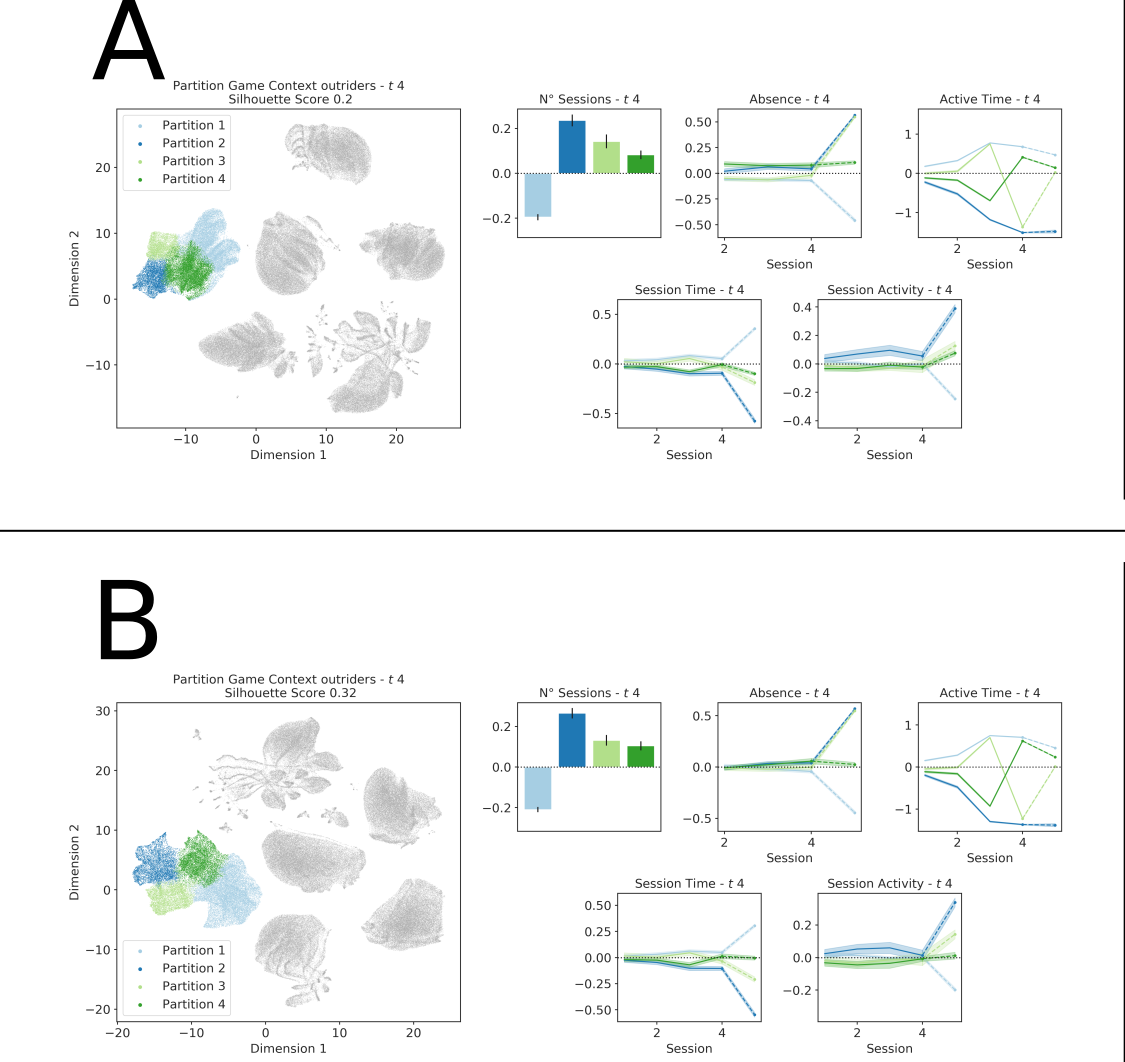
\includegraphics[width=0.7\textwidth]{images/chapter_4/clust_beha.png}
\centering
\caption[Partitions of the representations generated by the RNN architectures from the behavioural metrics]{The two panels shows the individuated partitions and associated behavioural profiles at $t4$. The big panels report the same UMAP reduction presented in the last column of Figure \ref{full_panel_temporal}. Each dot is the representation associated with a particular individual and is colour coded based on the partition to which it belongs. Small panels represent the temporal evolution of the considered behavioural metrics for each individuated partition. The panel relative to N°Sessions only reports the prediction produced by the model as the number of preceding session is constant for all the partitions. The x axis reports the game sessions while the y axis the value assumed by the considered metric at a specific point in time. The y axis is expressed in terms of number of standard deviations from the game population mean (i.e. z-scores). Each line indicates the mean z-score while the shaded area around the line its 95\% confidence interval. The solid part of each line indicates the portion of the temporal series observed by the model (i.e. the input) while the dotted part the predictions produced at that point in time. The first columns shows the partitions associated with the representation extracted by the RNN architecture while the second those associated with the representation extracted by the version of the RNN architecture that included environmental and game events covariates. Each row reports the partitions individuated for the 6 considered game contexts.}
\label{partition_rnn_behaviour} 
\end{figure}

At a global level, the four partitions seem to belong to two general groups: a group with a high propensity to produce future interactions (i.e. partitions 1 and 2) and a group with low propensity (partitions 3 and 4). Noticeably, when looking in detail at each specific partition they appear as variations on the macro group they belong to. Interestingly the percentage of Session Time spent actively interacting with the game object (i.e. Active Time) and the expected N°Sessions seem to be a relevant components in this more granular characterization. 

We will now report examples of the type of behavioural "phenotype" that we were able to derive from the partition analysis. However, Given the unsupervised nature of the adopted methodology and the lack of any strong a-priori expectations on the profiles' outlook, we suggest to interpret them with cautions and consider them as the result of a purely exploratory analysis.

\paragraph*{\textbf{Partition 1}} represents individuals producing high intensity interactions (see Session Time) at a high frequency (see Absence). The high amount of Active Time highlights how the individuals were actively interacting with the game object. The individuals in this partition are projected to produce a number of future interactions that is below average while maintaining a high intensity profile. It can be speculated that the history of high intensity interactions reflected a positive propensity towards the game. This might have prompted individuals in this partition to consume most of the available contents in the game leading to a reduced amount of expected future interactions (i.e. N° Sessions).

\paragraph*{\textbf{Partition 2}} describes individuals that have a history of very infrequent (see Absence) and brief interactions with burst of activities and long idle times (they have the lowest Active time among the individuate partitions). These individuals are expected to maintain this trend in the future although producing a number of interactions that is largely above the average. An hypothetical explanation might see individuals in this partitions constituting a variant of those in Partition 1. The high frequency and intensity of interactions could suggest an eagerness to interact with the game object. This, combined with the low amount of consumed content (see Session Time and Active Time) could explain the projected high amount of future interactions.

\paragraph*{\textbf{Partition 3}} includes individuals whose interactions have been very frequent and average both in terms of length and amount of activity until session 3. From there, a burst in both the length and active time can be observed concomitant with a reduction in latency before the following interaction. This is followed by a re-bounce effect with a marked reduction in the length and intensity of the next interaction. These individuals are predicted to produce a number of future interactions slightly above average while also maintaining a low intensity profile. These individuals might have started with a normal propensity towards the game which suddenly increased around session 3 and had a "physiological" downturn around session 4. 

\paragraph*{\textbf{Partition 4}} contains individuals producing the least intense and frequent interactions. With the only exception of a brief increase in active time around session 4. These individuals are estimated to produce a number of future interactions just above average while maintaining the original low intensity profile. These individuals started and maintained a low intensity profile, suggesting a negative propensity toward the game. 

It is interesting to note that despite the partitions individuated for the various game objects always show the two "macro groups" mentioned above, their finer grain characterizations (i.e. the behavioural profiles extracted from the partitions) vary between game contexts suggesting the presence of a possible interaction (see Appendix \ref{partitions_behavioural}).

Although the individuated profiles can provide valuable information on the behavioural "fingerprint" of group of individuals, the most relevant and reliable information can be found in the relationship between the considered metrics. We observe that Session Time and Session Activity are usually highly correlated. Low Absence seems to be a good indicator of the propensity to produce more interactions in the future. Similarly, high Absence seems to be associated with a general history of low intensity interactions. It is also worth noting that variations in this metric seem to follow and be proportional to increases and decreases in interactions' intensity. 

We can also notice how there is often (but not always) a very high correspondence between the profiles associated with the representations generated by the two versions of the RNN architecture. However, looking at the average silhouette score values, it seems that including environmental and game events covariates help deriving tighter and more consistent partitions. This might have been driven by a similar mechanism that we find in conventional linear models: by including appropriate covariates it is possible to obtain more reliable and robust estimates of a specific coefficient of interest \cite{gelman2020regression}.

\subsection{Partitioning the representation associated to the environmental covariates}
\label{partition_environment}
Looking at Figure \ref{partition_rnn_env} we can see the partitions individuated by the Mini-Batch K-Means for the representation generated from the environmental metrics. Given that all the entries included in our dataset were logged using the same time zone (i.e. CEST) we decided to focus in this analysis only on individuals playing from Central European countries. By looking at Figure \ref{partition_rnn_env}A we can observe how individuals tend to distribute their interactions with a game object differently depending on the day of the week or the hour of the day. This finding is not surprising but is in line with the idea mentioned in sections \ref{estpred_motivation_engagement} and \ref{modelling_env_and_game_elements}: the environment in which an interaction (here, between an individual and a game object) occours contribute in determining its observed behavioural intensity. 
\begin{figure}[!htb]
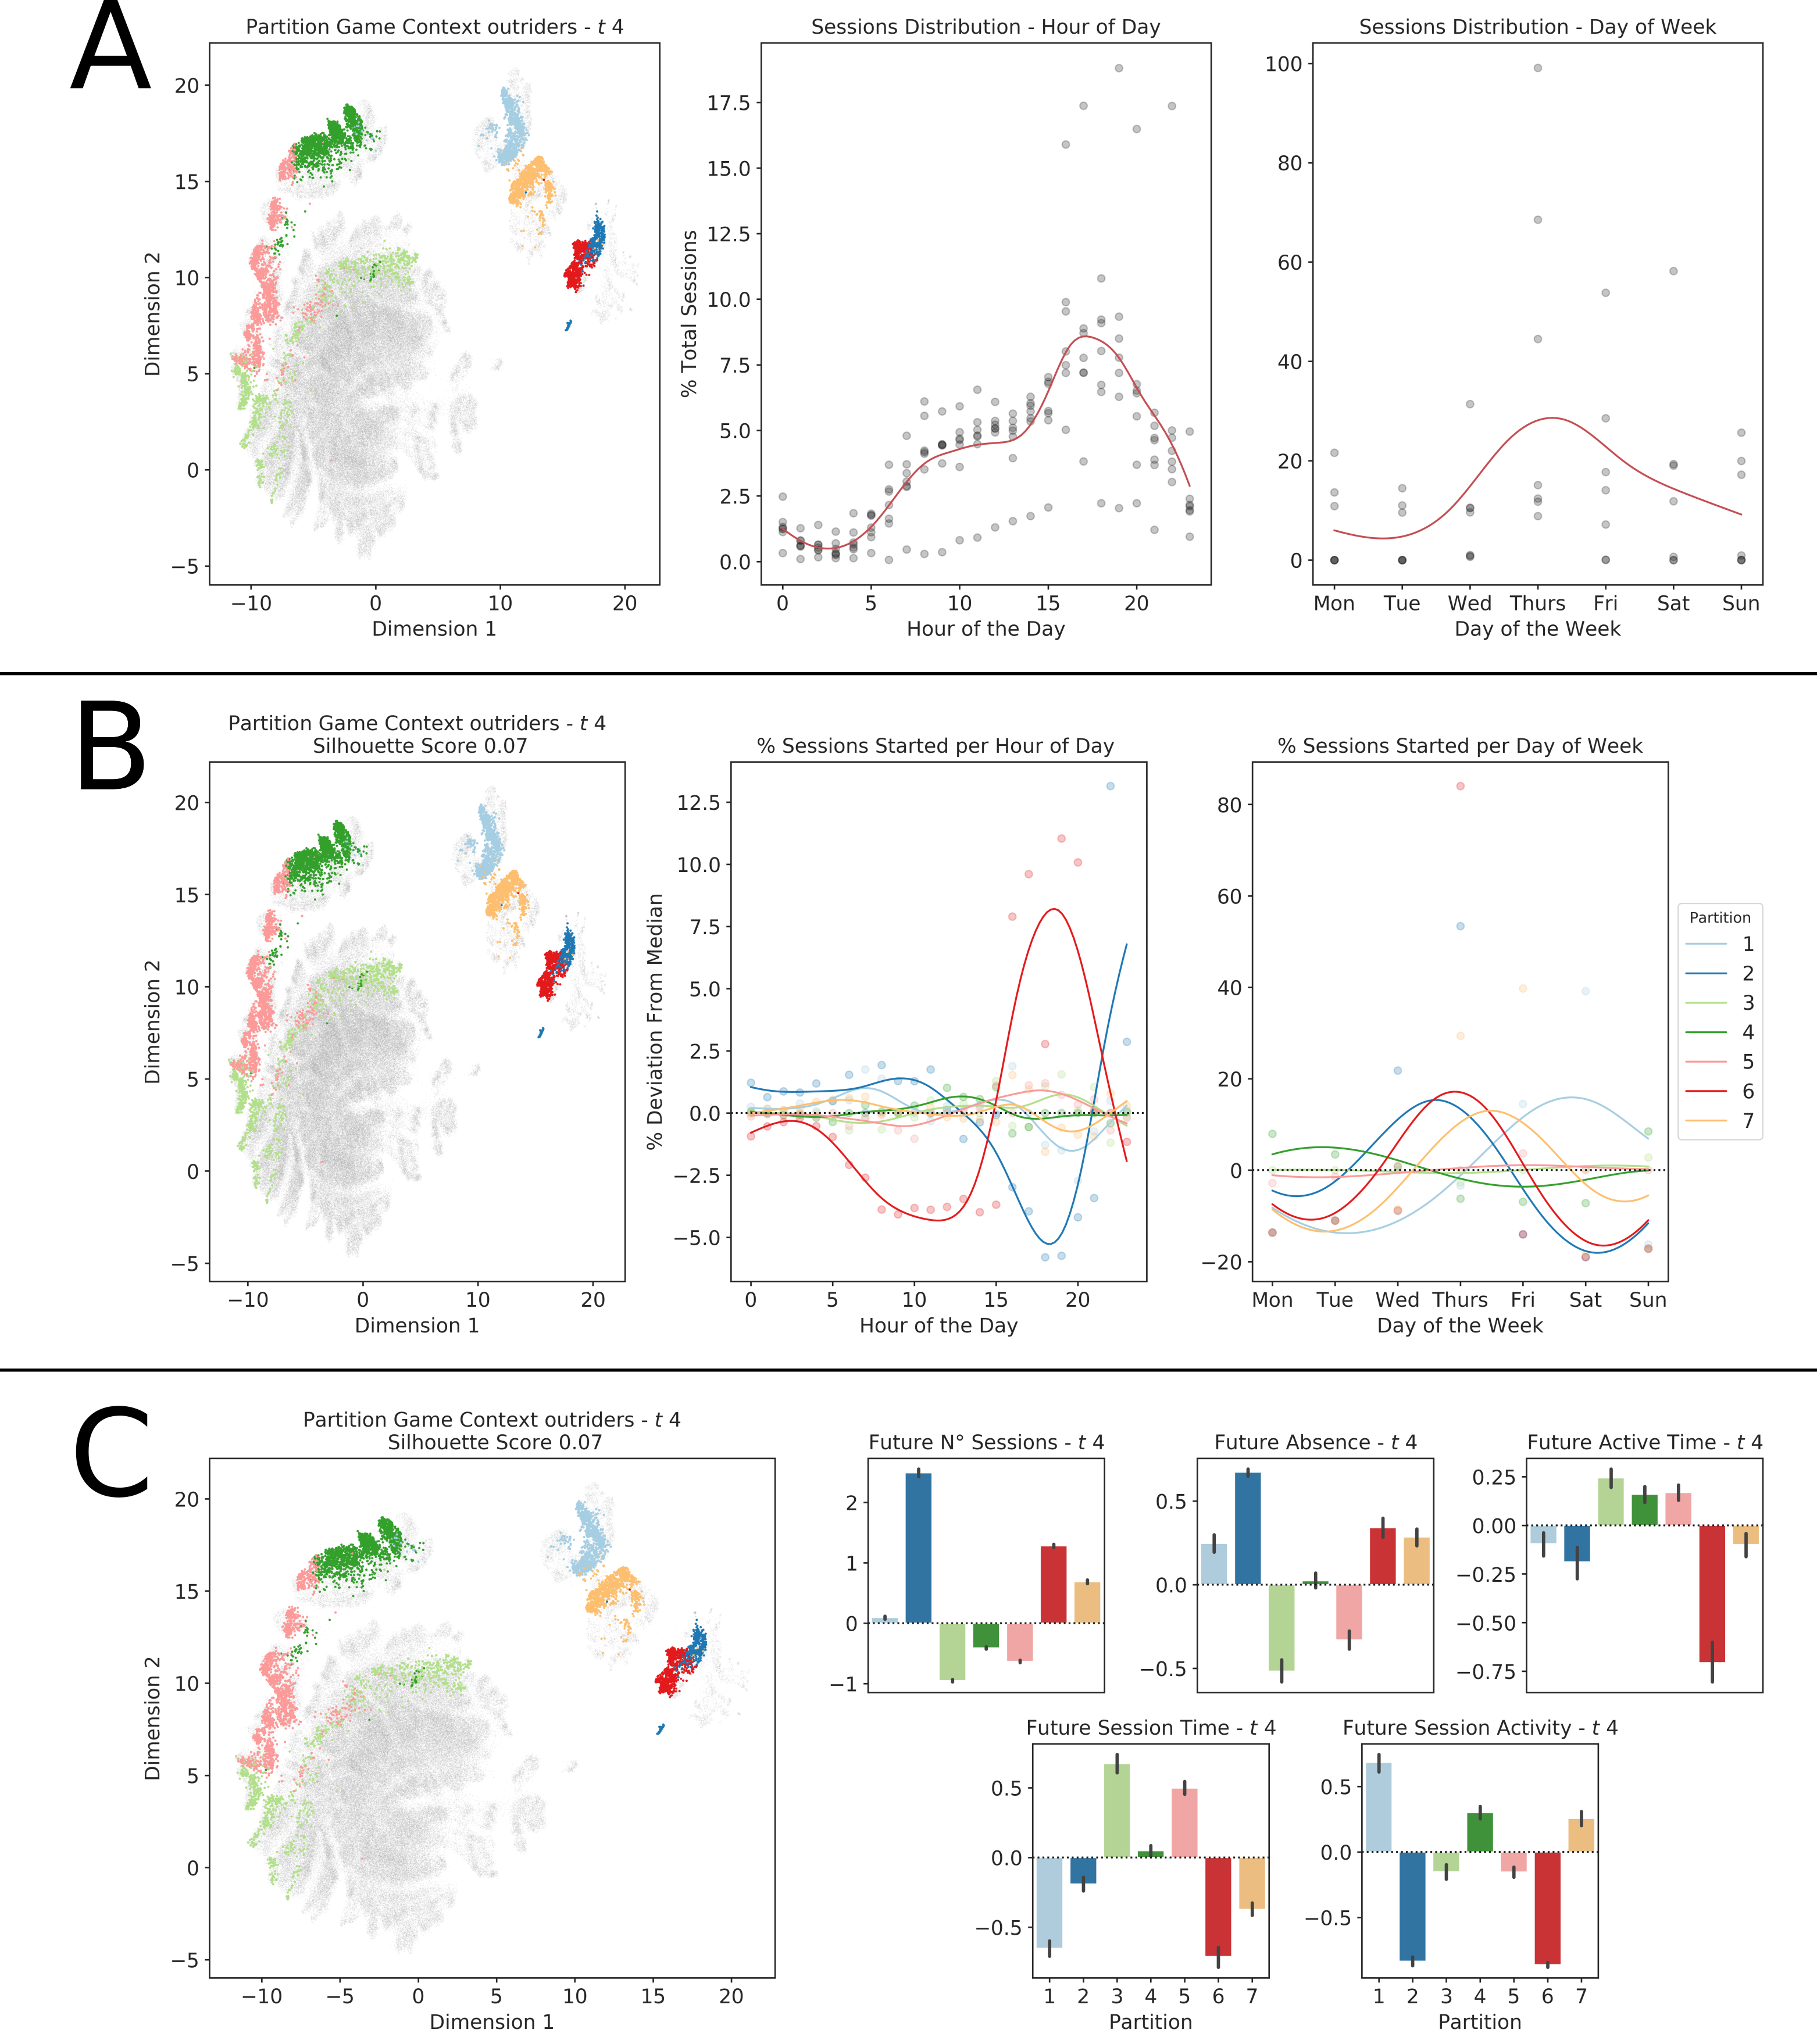
\includegraphics[width=\textwidth]{images/chapter_4/clust_env.png}
\centering
\caption[\textbf{Partitions of the representations generated by the RNN architectures using the environmental metrics}]{The panels show the individuated partitions and associated profiles for the representation encapsulating all the environmental information up to $t4$. Each panel reports the conventional UMAP reduction of the inferred latent representation with the colours representing membership to a specific partition individuated by the Mini-batch KMeans. The other two plots in panels A and B represent the percentage of total sessions that each partition initiated during a specific hour of the day or day of the week. The x axis reports either the hour of the day or the day of the week while the y axis the share of initiated sessions. For each panel we reported the line of best fit provided by a generalized additive model \cite{serven2018}. Panel A shows how each partition distributes its game sessions between different parts of the days or days of the week while panel B provides the same information at the sample level integrating over all partitions. The y axis in panel A is expressed in number of standard deviations from the sample mean. Panel C shows, similarly to Figure \ref{partition_rnn_behaviour} , differences in the predictions produced by the model for each partitions. The x axis indicates the partition number while the y axis the expected prediction made for a specific partition. The y axis is expressed in terms of number of standard deviations from the sample mean (i.e. z-scores) with black line indicating the 95\% confidence interval}
\label{partition_rnn_env} 
\end{figure}

Looking at Figure \ref{partition_rnn_env}A we can observe that the amount of playing activity in the considered sample tends to grow monotonically (but not linearly) from early in the morning (roughly around 6 a.m.) until early in the evening, peaking at around 7 p.m. A finding that is compatible with the expected daily schedule and circadian rhythm of individuals in the considered regions \cite{vitaterna2001overview} and with the results obtained by Vihanga and colleagues \cite{vihanga2019weekly}. A similar pattern can be observed for the distribution of playing activity during the days of the week: starting from Monday, individuals seem to progressively initiate more game sessions over time with peak activity recorded between Thursday and Friday. 

Interestingly, it appears that the nature of the object (i.e. the game context) plays a role in determining how different environmental factors influence the intensity of the interactions. A finding that is in again in line with the work of Vihanga and colleagues \cite{vihanga2019weekly, wannigamage2021player}. Looking at the Figures in Appendix \ref{partitions_environmental}, we can see for example that the game object $hmg$ shows a different distribution of playing sessions during the hours of the day with respect to $outriders$. For $hmg$ sessions seem to be roughly equally distributed during the day while for $outriders$ they peak towards the end of the day. This might be explained by the fact that being $hmg$ a mobile game, it allows individuals to  more easily initiate playing sessions at any moment during the day. In other words, the considered environmental factors would be posing less constrains on the intention to initiate the gaming activity. This type of differences appear even more pronounced and pervasive when looking at the distribution of playing sessions over the days of the week. 

More nuanced differences appear to emerge when inspecting the profiles derived by the partition analysis. Looking at Figure \ref{partition_rnn_env}B we can see how different groups of individuals distribute their playing activity differently in a way that is not necessarily compliant with what emerged from Figure \ref{partition_rnn_env}A. Like in the case of the behavioural profiles we suggest to interpret these findings with cautions and consider them as a descriptive rather than prescriptive device. 

\paragraph*{\textbf{Partitions 3, 4 and 5}} represent individuals with a distribution pattern which is not radically different from what observed in Figure \ref{partition_rnn_env}A. Partitions 3 and 5 show a slight preference for evening rather than morning interactions while the opposite is true for partition 4 which seems to also have initiated more playing sessions at the beginning of the week. They are expected to have a number of future playing sessions below average, but their next interaction is expected to be of moderately high intensity and to occur in a short amount of time. These individuals might have had a regular schedule of relatively long playing sessions that allowed them to consume a considerable amount of in-game content.

\paragraph*{\textbf{Partitions 1 and 7}} include individuals showing a slight preference for early morning rather than evening interactions. Partition 7 appears to have initiated more sessions late in the week (e.g. Thursday and Friday) while partition 1 seems to have favoured the weekend. The profile emerging from the expected intensity of their next interaction appear to be similar for both partitions: a brief but intense session occurring after a relatively long hiatus. These individuals might have had only a relatively narrow window of time for accumulating their playing activity.  Nevertheless they are expected to keep interacting with the game object (see the expected Future N° Sessions) suggesting that, despite the environmental constrains, they might be attributing high value to the playing activity.

\paragraph*{\textbf{Partitions 2 and 6}} are the ones showing the most unusual and extreme patterns. Individuals belonging to partition 2 appear to have initiated most of their session very late at night or very early in the morning avoiding the afternoon and evening. Partition 6 shows the opposite patterns, with playing sessions happening exclusively between late afternoon and early in the evening. Both profiles appears to have logged most of their activity in the middle of the week at the expenses of the weekend. The next session for these individuals is expected to be brief, of low intensity and occurring after a relatively prolonged period of time. However, these partitions encompass individuals that are expected to have the highest number of future playing sessions. This suggest that, similarly to what we observed for partitions 1 and 7, these individuals might have enjoyed the playing activity but the manifestation of their playing behaviour has been hampered by environmental constrains.

The results of this partition analysis, in conjunction with what emerged in sections \ref{results_3} and \ref{representation_env_even_contr} seems to support our intuition regarding the role of environmental covariates in the representation generated by the RNN architecture. 

These type of factors might influence the intensity of future interactions that an individual has with a particular game object however acting mostly as facilitators or impediments to the observed behaviour (see partitions 2 and 6) rather than inherently influencing the internal state of the individual. 

Indeed, differently from what we can observe in Figures \ref{rnn_env_even_full_events} and \ref{rnn_env_even_full_beha}, the representation extracted by the environmental encoder appears unable to clearly distinguish between individuals based on the expected intensity of their future interactions. Interestingly, the results of the partition analysis show that the representation is not just noise but can be used for discerning different patterns of interactions. This suggest that despite the model was able to organize information so to capture similarities between interaction patterns, this might not have been crucial for the minimization of the model objective, or at least not in the same way as behavioural and game events covariates showed to be.

The only notable exception to this seems to be when environmental covariates describe unusual and exceptional situations (e.g., partitions 2 and 6). The reason might be that in these cases there is a correspondence between the environmental conditions in which an interaction occurred and the expected intensity of the next one. For example, speculating that individuals in partition 2 might be doing some form of shift work that allows them to play only late at night or early in the morning, it is reasonable to expect their future interactions to be of low intensity. This is because there is a consistent constrain on how much time they can dedicate to the playing activity, regardless of how enjoyable they might find it.

\subsection{Partitioning the representation associated to the game events covariates}
\label{partition_event}
\begin{figure}[htbp]
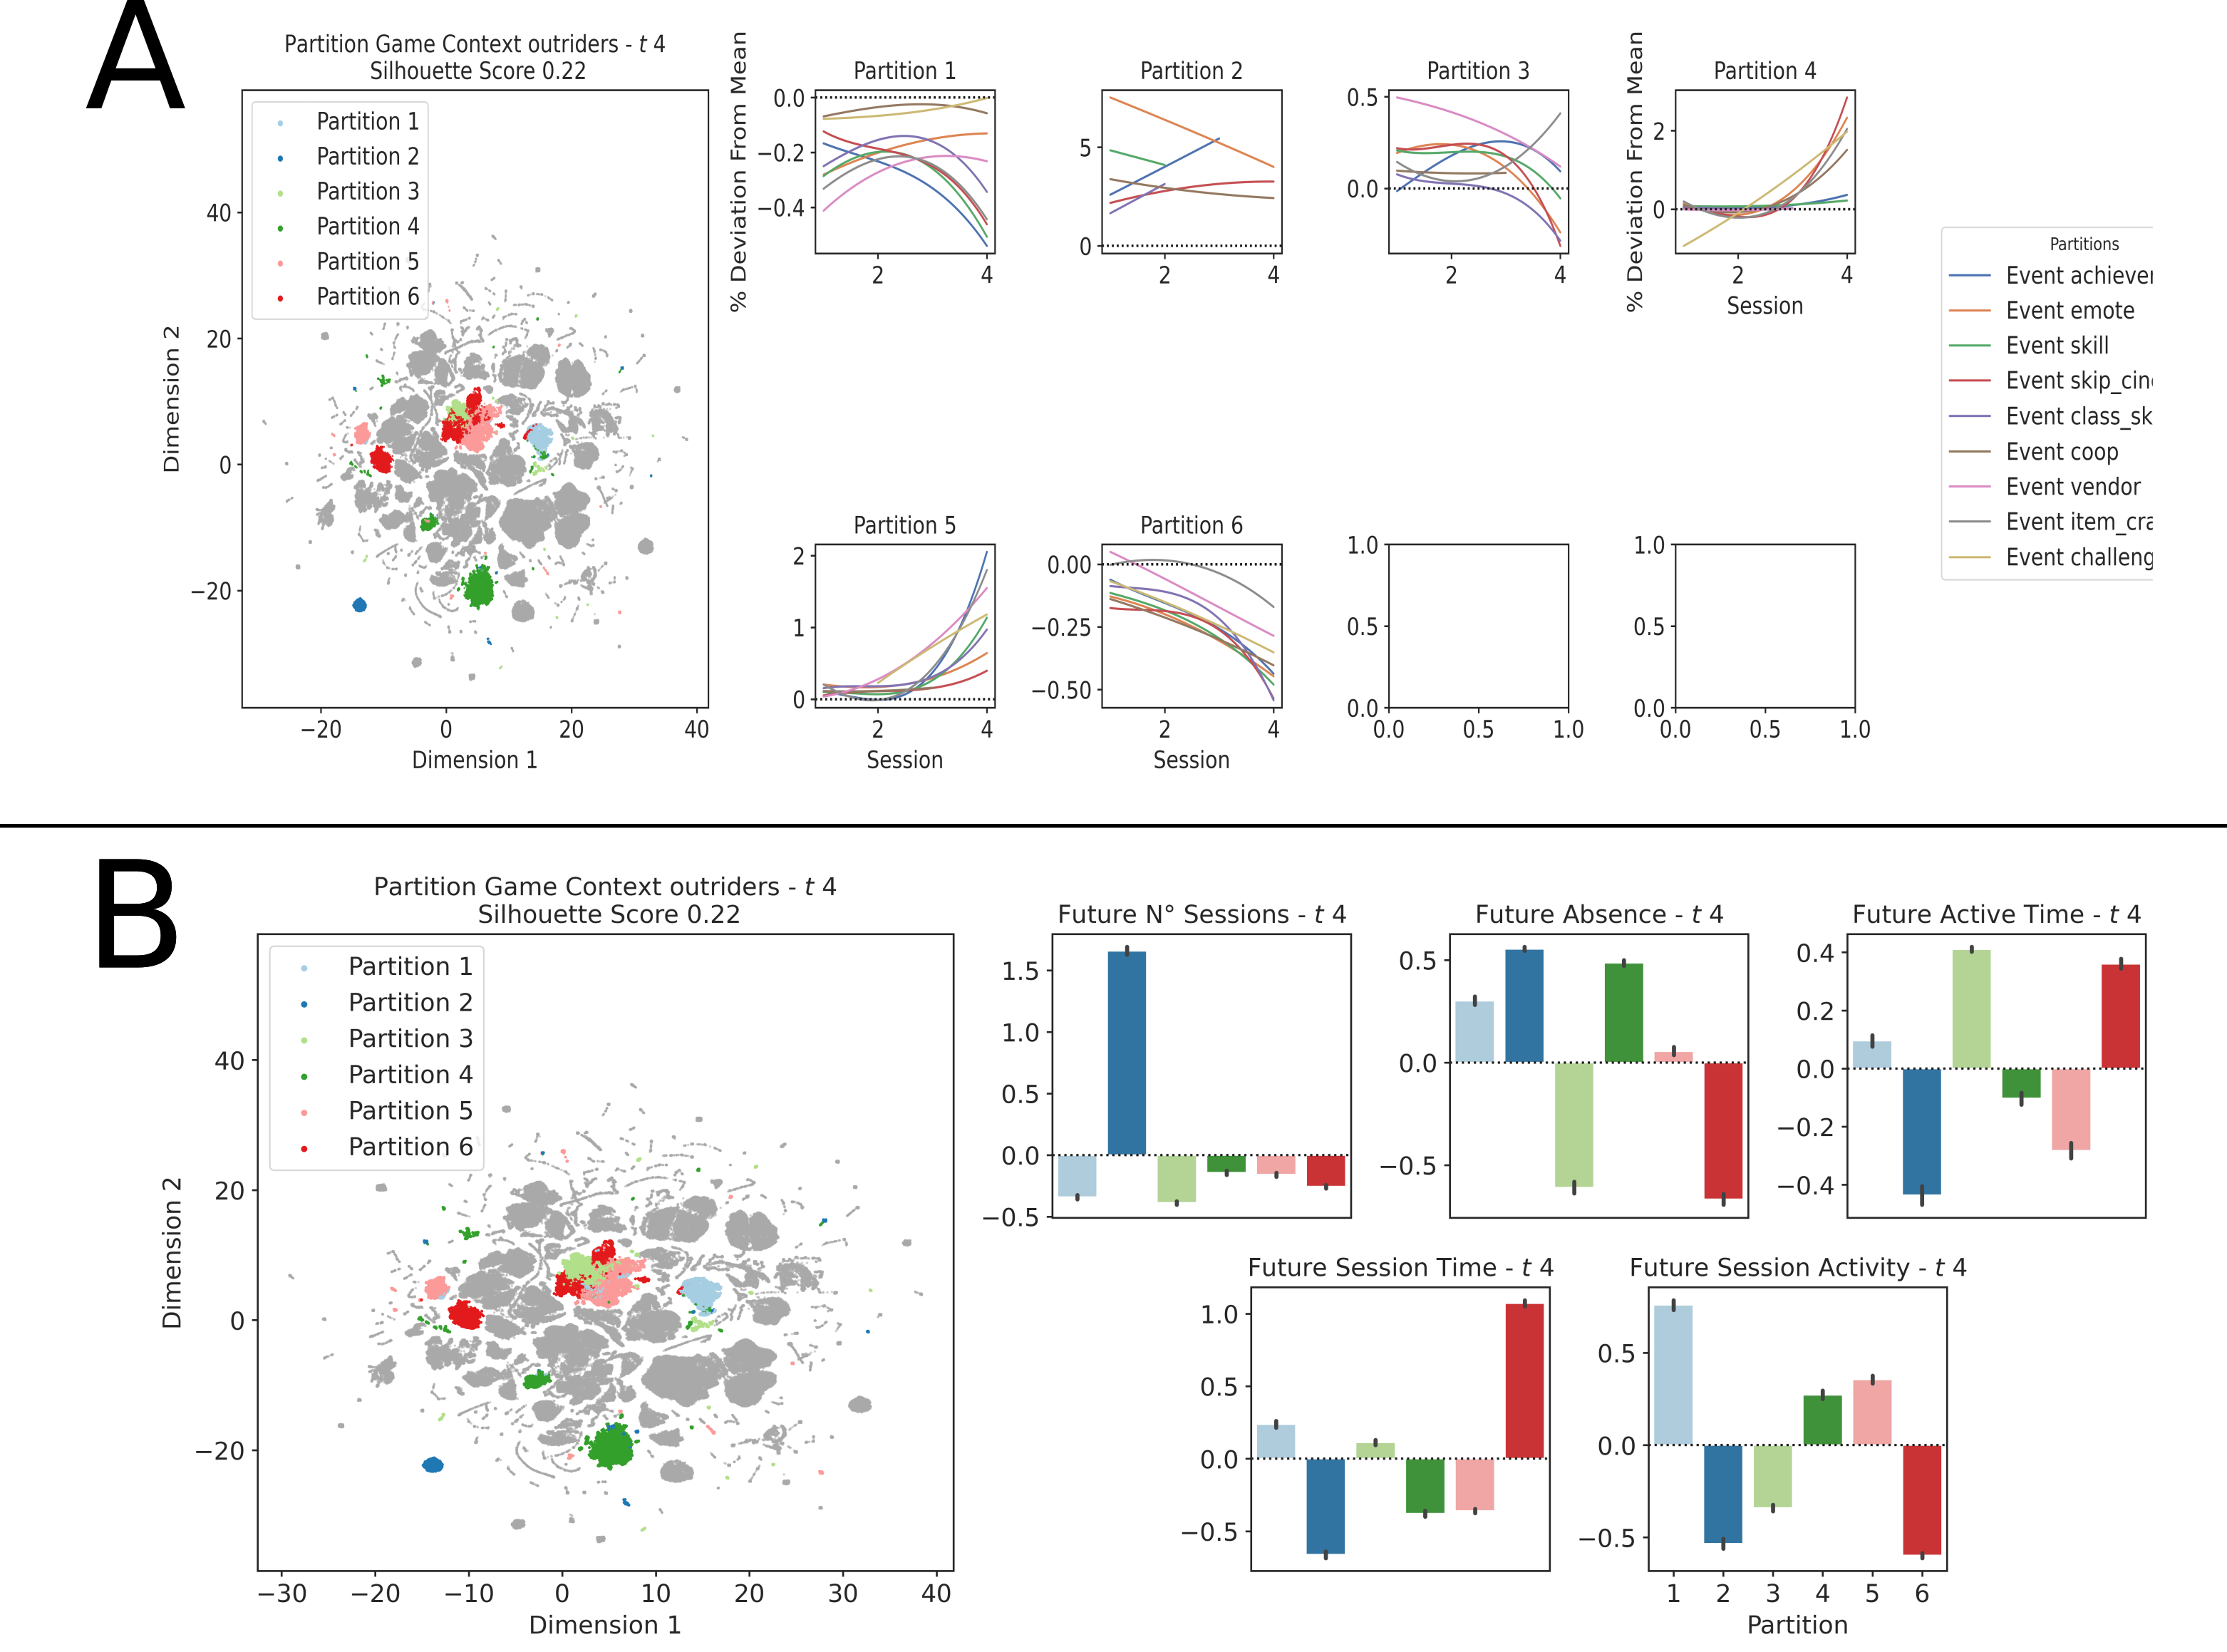
\includegraphics[width=\textwidth]{images/chapter_4/clust_even_outr.png}
\centering
\caption[Partitions of the representations generated by the RNN architectures from the game events metrics]{Panels show the individuated partitions and associated profiles for the representation encapsulating all the game events information up to $t4$. Each panel reports the conventional UMAP reduction of the inferred latent representation with the colours representing membership to a specific partition individuated by the Mini-batch KMeans. Panel A shows for each partition the share of events triggered during each considered game session expressed as number of standard deviations from the sample mean (i.e. z-scores). This information is conveyed through the line of best fit provided by a generalized additive model \cite{serven2018}. Panel C shows, similarly to Figure \ref{partition_rnn_behaviour} , differences in the predictions produced by the model for each partitions. The x axis indicates the partition number while the y axis the expected prediction made for a specific partition. The y axis is expressed in terms of number of standard deviations from the sample mean (i.e. z-scores) with black line indicating the 95\% confidence interval.}
\label{clust_even_outr} 
\end{figure}

\section{Discussion}
As mentioned in section  \ref{incentive_salience}, incentive salience attribution produces latent representations of objects that, when imbued with value, make future interactions with those objects more likely and intense \cite{berridge1998role,berridge2004motivation}. 

The fact that the representation generated by our model could be effectively described by a relatively small number of dimensions (potentially 2) appeared to be in line with this and compatible with the idea presented in section \ref{motivation} that motivation-related internal states can be compared to the magnitude of a 2-dimensional vector. This metaphor of the "motivational vector" seems to be compatible with the global-local organization of the representation generated by the RNN architecture and its improved version. 

At the global level, different game-objects were organized in distinct and coherent regions (see Figure \ref{full_panel_static}A) showing how the model attempted to operate on a meta-level by partitioning a global representation in several object-specific ones. This finding aligns with what highlighted in various work on neural manifold where the responses related to qualitatively different stimuli tends to show a cluster-like organization when reduced to a lower dimensional space \cite{stopfer2003intensity, gallego2017neural, ganmor2015thesaurus}. 

At the local level, each object-specific representation showed an internal gradient-like organization distinguishing individuals based on the estimated intensity of their future interactions with that specific object. This was true for each of the considered behavioural targets (see Figure \ref{full_panel_static}A) showing how the model attempted to provide an holistic description of the intensity of future interactions. The presence of this type of gradient-like organization emerged in a work by Nieh et al. \cite{nieh2021geometry} when analyzing neural responses during an evidence accumulation task in virtual reality. When reducing the neural activity to a 3 dimensional space, the resulting manifold presented a clear gradient able to code simultaneously for position and levels of accumulated evidence \cite{nieh2021geometry}. A similar finding was present in the work by Stopfner et al. \cite{stopfer2003intensity} where the manifold structure extracted from the activity of olfactory neurons was able to represent qualitative and quantitative differences between odours through a global-local organization similar to that showed in section \ref{functional_properties}.

The dynamic nature of the representation generated by our approach also nicely fits with that of attributed incentive salience \cite{toates1994comparing,robinson1993neural,zhang2009neural,tindell2009dynamic,berridge2012prediction}. In particular, the fact that the aforementioned global-local organization is maintained over time (see Figure \ref{full_panel_temporal}A) corroborate the hypothesis that our model approximated state changes originated from a dynamic process. In support of this, we also observed that the representation generated by our model was spatially coherent over time: it produced distinct regions of low and high expected intensity between which individuals moved over time (see Figure\ref{full_panel_temporal}D). These results appear to match the definition of motivation and incentive salience attribution specified in section \ref{motivation}: a single overarching process able to dynamically predict the likelyhood and intensity by which individuals will interact with a varied set of objects \cite{simpson2016behavioral,toates1994comparing,berridge2004motivation,zhang2009neural}. 

Many other cognitive and affective functions might rely on a latent representation that is functionally similar to the one described in our work (e.g. credit assignment and optimal control \cite{wang2018prefrontal, barto2004reinforcement}, cognitive control, learning \cite{skinner1965science} or various forms of reward processing \cite{schultz1997neural, schultz2000reward}). Similarly to attributed incentive salience, these functions are all involved in generating motivated behaviour and heavily rely on reward signals, however none of them is concerned with attributing and describing the motivational saliency that an object possess. This is made evident in the works by McClure et al. \cite{mcclure2003computational} and Zhang et al. \cite{zhang2009neural} where the system involved in salience attribution is functionally separate from the one assigning credit and executing actions: the former provide a representation that informs and biases the decisions taken by the latter serving an almost exclusively qualifying role (see the role of attributed incentive salience in addiction-like conditions \cite{robinson1993neural}). Similarly, the representation generated by our model doesn't provide any insight on the decision making process underlying the observed playing behaviour but simply provide an approximate description of the "motivational pull" that a particular game object has on a particular individual at a certain point in time. 

The functions encoded by the hidden units constituting the representation appeared to have a series of distinctive properties, namely: redundancy, non linearity, multiplicity (single units code for multiple functions) and consistency over time. These may have played a role in providing the representation generated by our model with its distinctive characteristics. For example, as we mentioned in section \ref{manifold_rep_incentive_salience} redundancy and inter-correlation are characteristics of the signals from which the manifold representation of internal states arises \cite{seung2000manifold,gallego2017neural}. Multiplicity on the other hand, might be the factor underlying the ability of our model to produce a single unitary representation which holds predictive power over different behavioural targets. Finally, consistency over time could be the mechanisms supporting the type of temporal coherence observed in panel \ref{full_panel_temporal}D. We want to stress that these findings are to be considered exploratory in nature since they do not rely on a-priori hypotheses. A comparison between these computational properties and those underlying the attribution of incentive salience is required and would constitute a potential venue for future investigations. 

The introduction of environmental and game events covariates appeared to have produced a more consistent representation (see Figures \ref{rnn_env_even_full_shared} \ref{rnn_predictive_comparison}) with better discriminatory powers, a finding in line with the, although marginal, improvements in predictive perfromance observed in section \ref{results_3}. It might be speculated that this improvement was associated both with the introduction of new informative covariates and with the ability of the architecture to separately model their contribution. Indeed, similarly to the idea underlying Neural GAMs \cite{agarwal2021neural}, different portion of the architecture might have focused on inferring specialized functions then combined in a more effective latent representation.

However, the major advantage provided by separately modelling the contribution of behavioural, environmental and game-events metrics lied in the ability to obtain distinct representations that we were able to leverage for exploratory analyses. This allowed us to perform time series partitioning at a much larger scale that has been previously done in the videogames literature (potentially up to millions of time series) \cite{bauckhage2014clustering, makarovych2018like, vihanga2019weekly, aung2019trails}. Indeed, previous approaches in the literature attempted to cluster or partition directly the observable data space, a particularly cumbersome process for univariate and multivariate time series, especially if suitable techniques like Dynamic Time Warping \cite{muller2007dynamic} are to be used. In our case by leveraging the representational power of ANNs we were able to condense the information present in the the time series data to a more compact representation, this allowed us to then rely on relatively inexpensive algorithm (i.e. Minini-Batch KMeans) for performing the partitioning.

The partition analysis conducted on the behavioural representation allowed to individuate a set of profiles that are, to a certain extent, consistent with behavioural correlates of different levels of attributed incentive salience \cite{berridge2004motivation} and general operant conditioning principles \cite{thorndike1927law, skinner1953science, nevin2000behavioral}: the strength of past interactions positively correlate with the frequency and intensity of future ones. The various offsets that each partition showed might suggest different levels of predisposition towards the various game-objects. The dynamic nature of these profiles provided a more granular characterization allowing to observe variations in the entire history of interactions and not just in the expected intensity of future ones. For example, it was possible to see how a higher likelihood of future interactions was supported both by a history of low intensity but high frequency interactions as well as by a series of high frequency and high intensity interactions. In this sense, these behavioural profiles can be seen as useful devices for investigating the existence of inter-individual differences in schedules of interactions with potentially rewarding objects. 

On the other hand, partitioning the environmental representation provided us with insights on how different individuals distributed their interactions with a videogame over days of the week and hours of the day. We were able to replicate some of the findings of Vihanga and colleagues \cite{vihanga2019weekly, wannigamage2021player} individuating similar profiles of interactions. However, our approach allowed us to gather insights not just on the characteristics of the different profiles but also on their potential impact on interaction intensity.

\subsection{Limitations and Future Work}
Despite our findings seem to suggest a similarity between the functional characteristics of the representation inferred by our approach and the construct of attributed incentive salience these are the result of mostly qualitative, descriptive or exploratory analyses. 
Since our approach is attempting to solve an inverse problem, the issue of uniqueness arises. Many different latent states might have produced the behavioural patterns that our model observed and there is no guarantee of a strict one-to-one mapping between the representation generated by our model and attributed incentive salience.  More effort should be posed in future research for obtaining a clear formulation of the computations carried out by our architectures. Alternatively, an extensive work of validation could be carried out by comparing the representations generated by our architectures with those generated from data gathered through laboratory or simulation experiments. 

The behavioural profiles individuated by our partition analyses seem to overlap with other findings in the literature however some results appeared unexpected and potentially contradictory. Given the observational setting of our work and the unsupervised approach we adopted, the explanations provided in section \ref{partition_analysis} should be taken with caution and be seen as a method for generating testable hypotheses that should constitute the starting point for future investigations. Indeed, clarifying the the nature of some of the observed discrepancies may require experimental work in more controlled settings. Lastly, despite our approach appeared to deal gracefully with objects having different structural characteristics, these were limited to the domain of video games. In order to verify the generalizability of our approach, future work should include data generated from a variety of contexts (e.g. web services, online and laboratory-based experiments).  